\documentclass[pdf,notes]{beamer}
\usetheme{Copenhagen} % For colored blocks
\setbeameroption{hide notes} % Only slides
% \setbeameroption{show notes on second screen=bottom} % Both

%\documentclass[aspectratio=169]{beamer} % 16:9
\usepackage{ctex, hyperref}
\usepackage[T1]{fontenc}
\usepackage{bm}

% other packages
\usepackage{latexsym,amssymb, amsmath, amsfonts,xcolor,multicol}
\usepackage{graphicx,pstricks,listings,stackengine}
\usepackage{ragged2e} % For text alignment
\usepackage{mathtools}
\usepackage{tabularx}
\usepackage{booktabs} % For prettier tables
\usepackage{colortbl} % For row colors
\usepackage{xcolor}   % For color definitions
\usepackage[linesnumbered,ruled,vlined]{algorithm2e}

\author{Presented by: Camilo Martínez}
\title{Overview --- "Active Contours Without Edges"}
\subtitle{By Tony F. Chan, and Luminita A. Vese}
\institute{Universität des Saarlandes}
\date{June, 2024}
\usepackage{CNU}    

% defs
\def\cmd#1{\texttt{\color{red}\footnotesize $\backslash$#1}}
\def\env#1{\texttt{\color{blue}\footnotesize #1}}
\definecolor{deepblue}{rgb}{0,0,0.5}
\definecolor{deepred}{rgb}{0.6,0,0}
\definecolor{deepgreen}{rgb}{0,0.5,0}
\definecolor{halfgray}{gray}{0.55}

\lstset{
    basicstyle=\ttfamily\small,
    keywordstyle=\bfseries\color{deepblue},
    emphstyle=\ttfamily\color{deepred},    % Custom highlighting style
    stringstyle=\color{deepgreen},
    numbers=left,
    numberstyle=\small\color{halfgray},
    rulesepcolor=\color{red!20!green!20!blue!20},
    frame=shadowbox,
}

\setbeamercolor{emph}{fg=red} % Define a custom color for emphasis
\renewcommand<>{\emph}[1]{% 
  {\usebeamercolor[fg]{emph}\only#2{\itshape}#1}%
}
\newcommand{\bfit}[1]{\textbf{\textit{#1}}} % Bold and italic text

\begin{document}

\kaishu
\begin{frame}
    \titlepage
    \begin{figure}[htpb]
        \begin{center}
            
\includegraphics[width=0.4\linewidth]{images/uds-logo.png}
        \end{center}
    \end{figure}
\end{frame}

\begin{frame}
    \tableofcontents[sectionstyle=show,subsectionstyle=show/shaded/hide,subsubsectionstyle=show/shaded/hide]
\end{frame}


\section{Motivation}

\subsection{A (brief) Introduction to Image Segmentation}

\begin{frame}{A (brief) Introduction to Image Segmentation}
    \begin{itemize} % [<+-| alert@+>]
        \item One of the most widely studied problems in \emph{Computer Vision}.
        \item Applicable in \textbf{medical imaging}, \textbf{robotics}, \textbf{video surveillance}, \textbf{materials science}, \textbf{autonomous driving}, and many others.
    \end{itemize}
    \begin{center}
        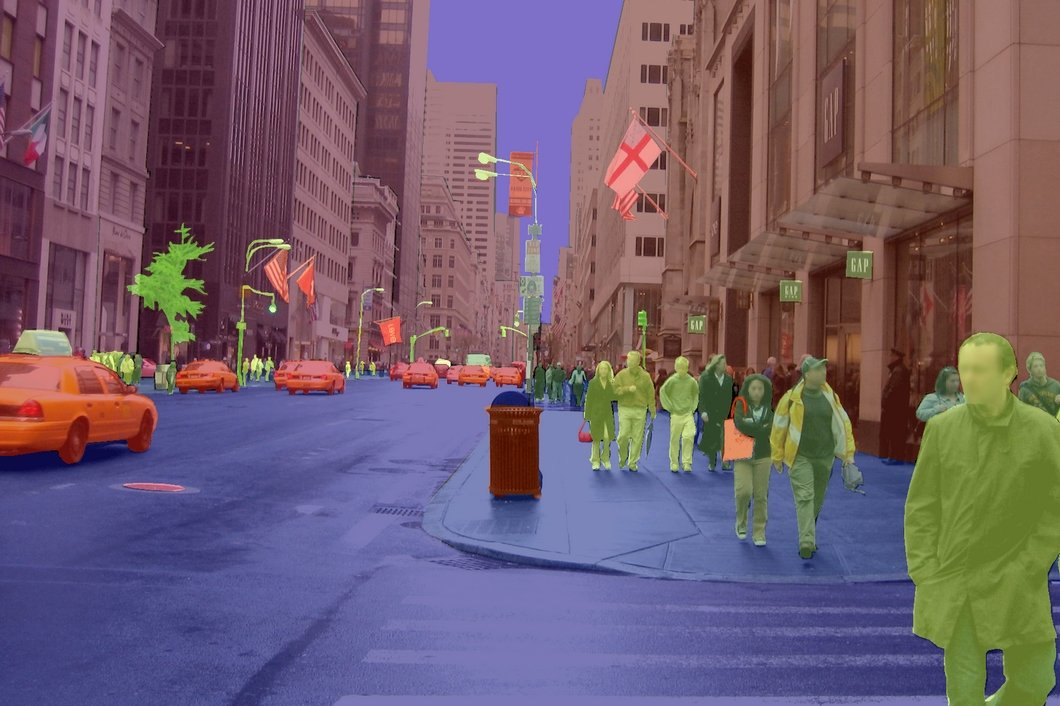
\includegraphics[width=0.7\textwidth]{images/introduction-autonomous-driving.jpg}
    \end{center}
    \vspace{-0.5\baselineskip}
    \centering
    \scriptsize Image segmentation in autonomous driving \cite{viso.ai} (2024).
\end{frame}

\begin{frame}{A (brief) Introduction to Image Segmentation}
    \begin{center}
        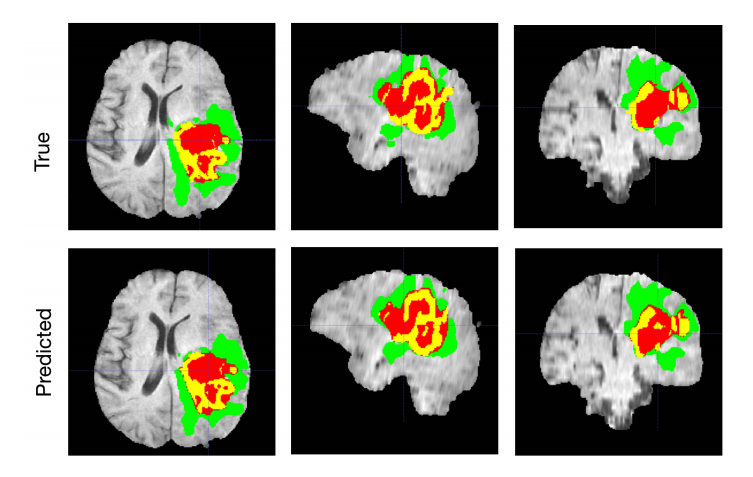
\includegraphics[width=0.9\textwidth]{images/introduction-tumor.png}
    \end{center}
    \vspace{-\baselineskip}
    \centering
    \justifying
    \scriptsize A typical segmentation example for \emph{tumor segmentation}. The predicted segmentation results match the ground truth well \cite{brats} (2018).
\end{frame}

\begin{frame}{A (brief) Introduction to Image Segmentation}
    \begin{minipage}{0.3\textwidth}
        \centering
        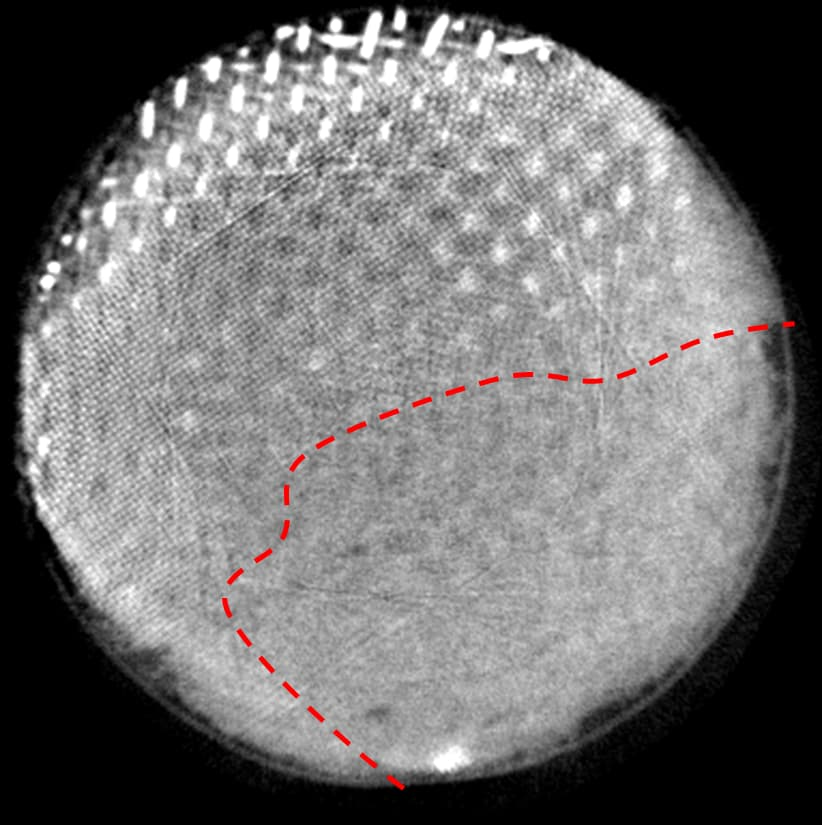
\includegraphics[width=\textwidth]{images/introduction-cylinder.jpeg}
    \end{minipage}
    \hfill
    \begin{minipage}{0.6\textwidth}
        \centering
        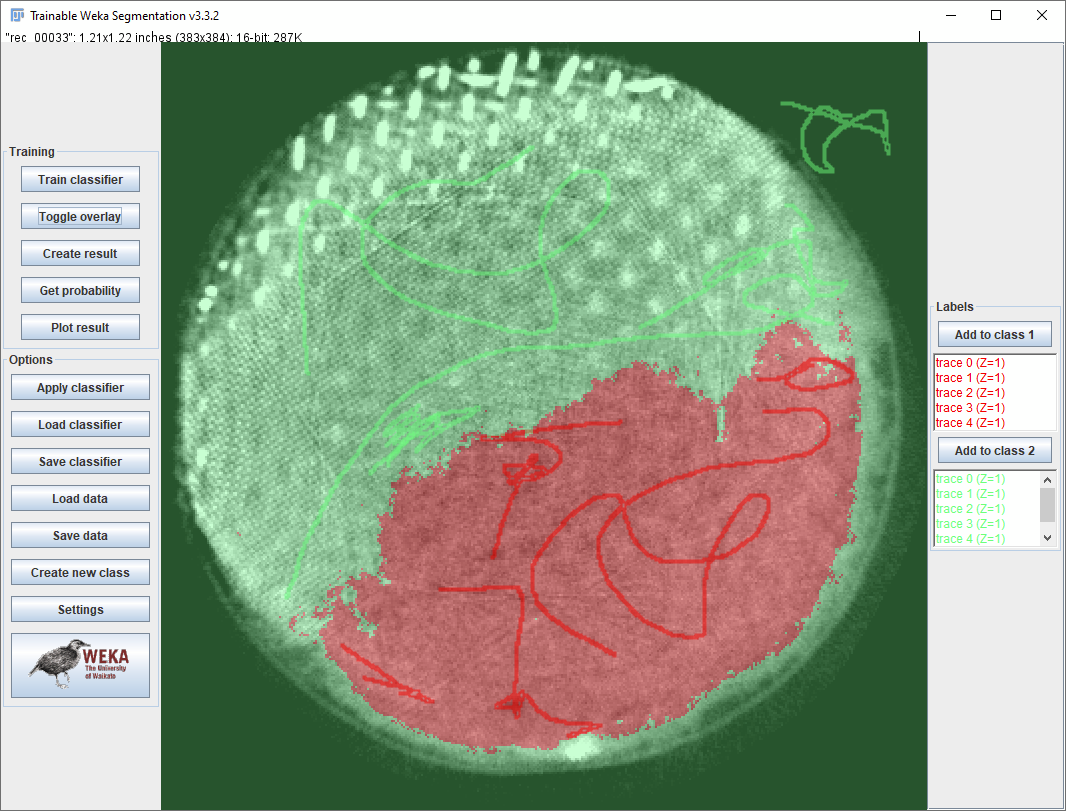
\includegraphics[width=\textwidth]{images/introduction-cylinder-segmented.jpeg}
    \end{minipage}
    \vfill
    \centering
    \justifying
    \scriptsize Slice of micro-CT of a solid cylindrical sample covered with a two metallic nets: inner is fine and outer is coarse. Segmentation done in \textbf{ImageJ}'s Trainable Weka Segmentation plugin \cite{imagej} (2022).
\end{frame}

\begin{frame}{A (brief) Introduction to Image Segmentation}
    \begin{minipage}{0.3\textwidth}
        \centering
        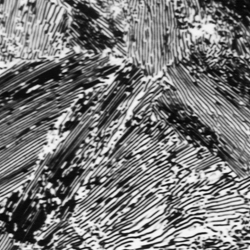
\includegraphics[width=\textwidth]{images/introduction-mechanical.png}
        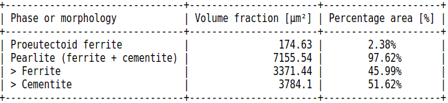
\includegraphics[width=\textwidth]{images/introduction-mechanical-properties-1.png}
        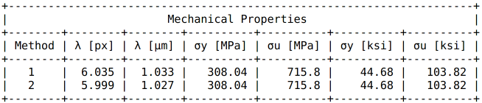
\includegraphics[width=\textwidth]{images/introduction-mechanical-properties-2.png}
    \end{minipage}
    \hfill
    \begin{minipage}{0.6\textwidth}
        \centering
        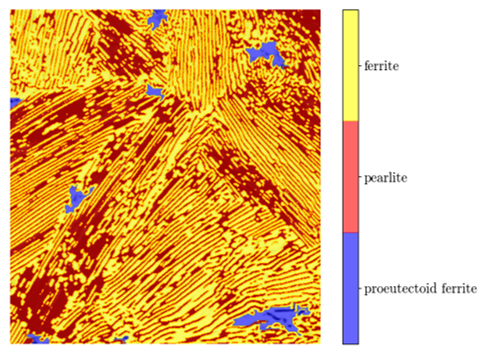
\includegraphics[width=\textwidth]{images/introduction-mechanical-segmented.png}
    \end{minipage}
    \vfill
    \centering
    \justifying
    \scriptsize Low-carbon steel microstructure, segmented into \textbf{ferrite} and \textbf{pearlite} phases. The segmentation results are used to calculate the mechanical properties of the material \cite{yo} (2021).
\end{frame}

\subsection{Predecessors to the Chan-Vese Model}

\begin{frame}{Predecessors to the Chan-Vese Model}
    \begin{itemize}
        \item \textbf{Early methods}: thresholding, region growing, edge-based segmentation.
        \item \textbf{Improvements}: snakes and active contours models.
        \item Challenges \emph{so far}: segmentation without clear edges.
    \end{itemize}
    \scriptsize
    \begin{center}
        \rowcolors{1}{gray!25}{white} % Alternate row colors
        \begin{tabularx}{\textwidth}{X l l}
            \toprule
            \textbf{Title}                                                  & \textbf{Authors}       & \textbf{Year} \\
            \midrule
            Boundary detection by minimizing functionals \cite{MumfordShah} & D. Mumford and J. Shah & 1985          \\
            Snakes: Active contour models \cite{Kass1988}                   & M. Kass et al.         & 1988          \\
            A topology independent shape modeling scheme \cite{Malladi1993} & R. Malladi et al.      & 1993          \\
            On geodesic active contours \cite{Caselles}                     & V. Caselles et al.     & 1997          \\
            \bottomrule
        \end{tabularx}
    \end{center}
\end{frame}

\begin{frame}
    \begin{center}
        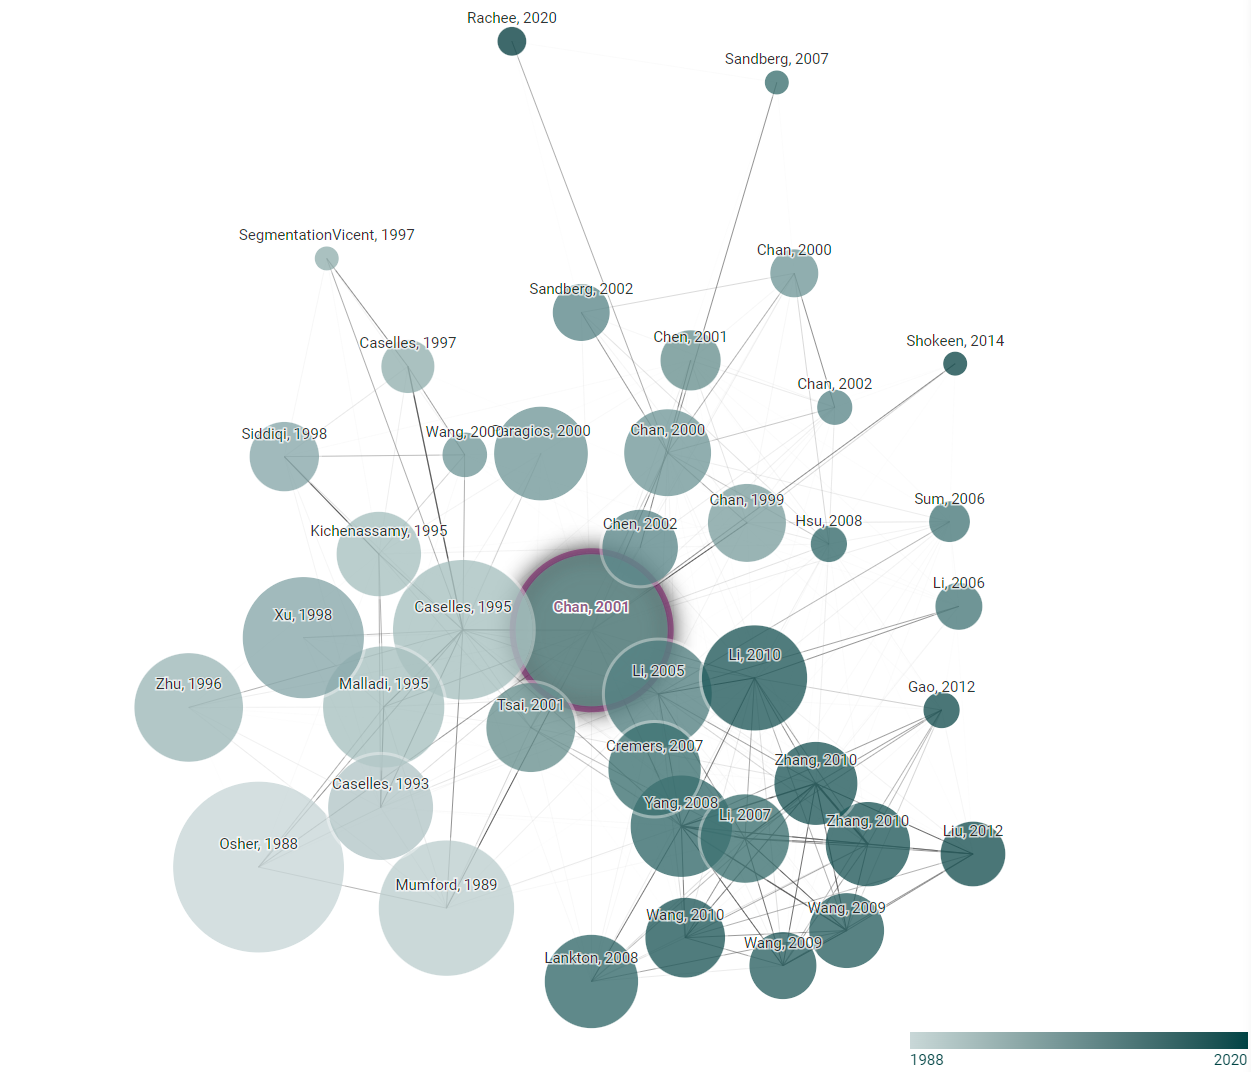
\includegraphics[height=0.9\textheight]{images/paper-graph.png}
        \vfill
        \scriptsize Prior and Derivative Works of the Chan-Vese Model. Courtesy of \href{https://www.connectedpapers.com/}{@ConnectedPapers}, this graph available \href{https://www.connectedpapers.com/main/3bdcc6c663112ab10ffb5b5e875f8e2660cd5001/Active-contours-without-edges/graph}{here}.
    \end{center}
\end{frame}

\section{The Chan--Vese Model}

\subsection{The "Fitting" Problem}

\begin{frame}{The "Fitting" Problem}
    \begin{itemize}
        \item \textbf{Chan and Vese (2001)} proposed a specific region-based active contour model, where the image is segmented into \textbf{two phases/regions}: object and background.
        \item Assume we have an image \( u({\bm{x}}), \bm{x} \in \Omega \), and the image is formed by two regions with mean intensity values: \( u_{in} \) and \( u_{out} \).
        \item Our \textit{evolving} boundary curve \( C \) separates the two regions.
        \item Then, we can define a \emph{fitting} term that penalizes deviations from the mean intensity values:
    \end{itemize}
    \vspace{\baselineskip}
    \[
        \textrm{fitting}(C) \coloneq F_{in}(C) + F_{out}(C)
    \]
\end{frame}

\begin{frame}{The "Fitting" Problem}
    \centering
    \tiny
    \begin{tabular}{@{}>{\centering\arraybackslash} m{0.48\textwidth} @{} >{\centering\arraybackslash} m{0.48\textwidth} @{}}
        $F_{in}(C) > 0, F_{out}(C) \approx 0$, fitting $> 0$                                                                        & $F_{in}(C) \approx 0, F_{out}(C) > 0$, fitting $> 0$                                                                         \\
        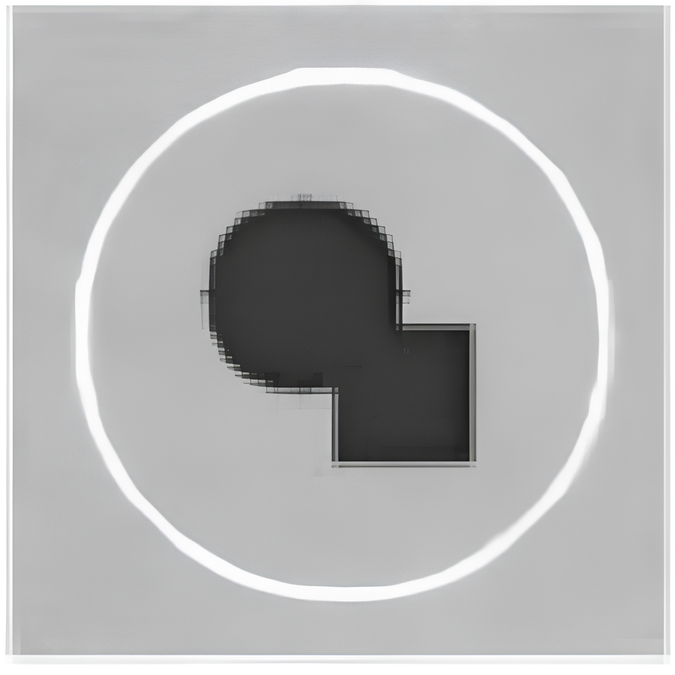
\includegraphics[width=0.35\textwidth,height=0.35\textheight,keepaspectratio]{images/fitting-problem-upper-left.png} & 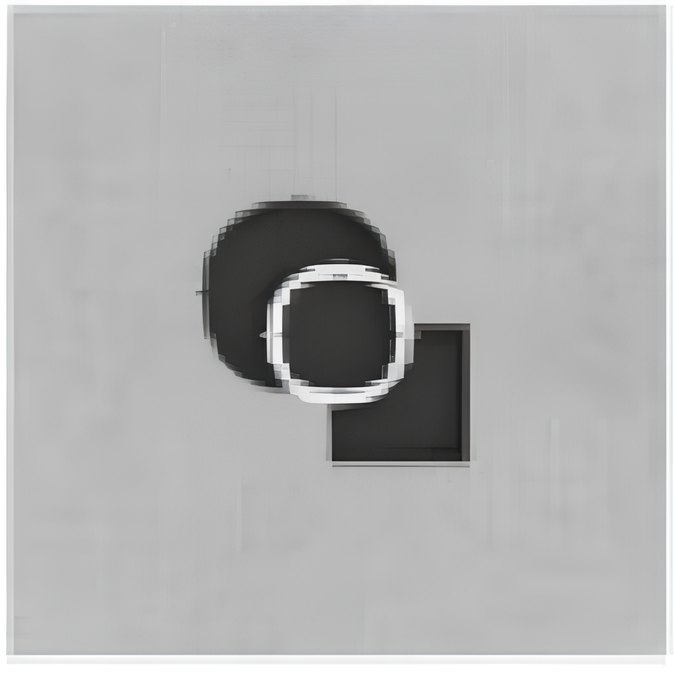
\includegraphics[width=0.35\textwidth,height=0.35\textheight,keepaspectratio]{images/fitting-problem-upper-right.png} \\
        $F_{in}(C) > 0, F_{out}(C) > 0$, fitting $> 0$                                                                              & $F_{in}(C) \approx 0, F_{out}(C) \approx 0$, fitting $= 0$                                                                   \\
        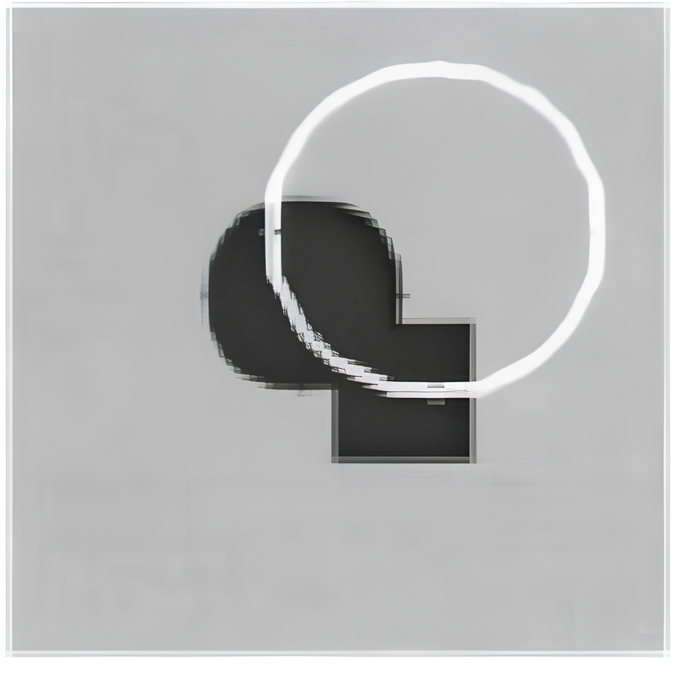
\includegraphics[width=0.35\textwidth,height=0.35\textheight,keepaspectratio]{images/fitting-problem-lower-left.png} & 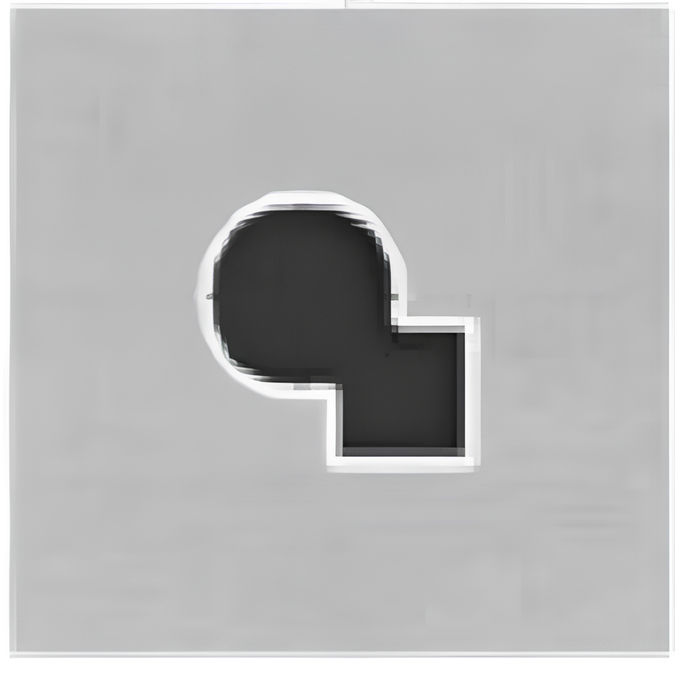
\includegraphics[width=0.35\textwidth,height=0.35\textheight,keepaspectratio]{images/fitting-problem-lower-right.png} \\
    \end{tabular}
    \vfill
    \justifying
    \scriptsize Consider all possible cases of $C$ enclosing the object in the image. The \emph{fitting} term is minimized only in the case when $C$ is exactly on the boundary of the object \cite{ChanVese}.
\end{frame}

\begin{frame}{The "Fitting" Problem}
    \begin{itemize}
        \item Furthermore, using a Mean-Squared Error (MSE) approach,
    \end{itemize}
    \begin{align*}
        \textrm{fitting}(C) & = \phantom{\int\limits_{inside(C)}} \color{blue}{F_{in}(C)} \phantom{\int\limits_{outside(C)}} \color{black}{+} \phantom{\int\limits_{inside(C)}} \color{red}{F_{out}(C)} \phantom{\int\limits_{outside(C)}}                                                                                                                                                 \\
                            & = \underbrace{\color{blue}{\int\limits_{\scriptscriptstyle inside(C)} |u(\bm{x}) - c_{in}|^2 \, d\bm{x}}}_{\text{\color{blue}{$> 0$, if $u(\bm{x})$ deviates from $c_{in}$}}} + \underbrace{\color{red}{\int\limits_{\scriptscriptstyle outside(C)} |u(\bm{x}) - c_{out}|^2 \, d\bm{x}}}_{\text{\color{red}{$> 0$, if $u(\bm{x})$ deviates from $c_{out}$}}}
    \end{align*}
    \begin{itemize}
        \item Thus, our minimizer $C_0$ that satisfies \(\textrm{fitting}(C_0) \approx 0\) can be defined as:
              \[
                  C_0 = \inf_C \{\textrm{fitting(C)}\} = \inf_C \{F_{in}(C) + F_{out}(C)\}
              \]
    \end{itemize}
\end{frame}


\begin{frame}{Formulation as an Energy Functional}
    \begin{itemize}
        \item We can introduce the energy functional $F(c_{in}, c_{out}, C)$ as:
    \end{itemize}
    \[
        F(c_{in}, c_{out}, C) = \underbrace{\color{purple}{\mu \cdot \textrm{Length}(C) + \nu \cdot \textrm{Area}(\textrm{inside}(C))}}_{\text{\color{purple}{penalize the "size" of $C$}}} + \textrm{fitting}(C)
    \]
    \begin{itemize}
        \item[] where $\mu, \, \nu \in \mathbb{R}_0^+$.
    \end{itemize}
    \begin{itemize}
        \item Thus, the minimization problem becomes:
              \[
                  C_0 = \inf_{c_{in}, c_{out}, C} F(c_{in}, c_{out}, C).
              \]
    \end{itemize}
    \begin{center}
        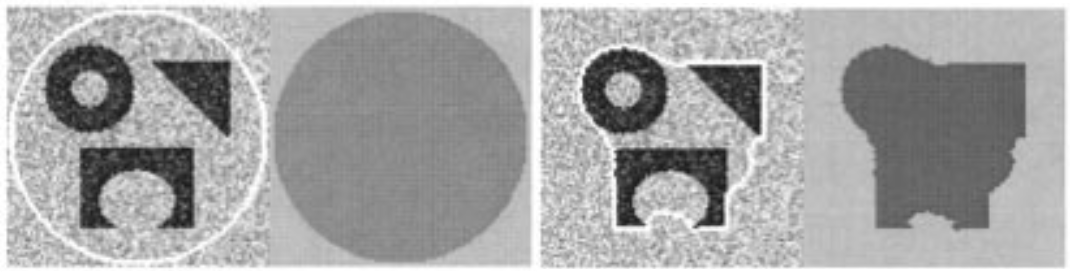
\includegraphics[height=0.2\textheight]{images/shrinking-illustration.png}
        \vfill
        \justifying
        \scriptsize Shrinking contour $C$, detecting different objects from a noisy image with various shapes. \textbf{Left:} $u$ and the contour. \textbf{Right:} the piecewise-constant approximation of $u$ \cite{ChanVese}.
    \end{center}
\end{frame}

\begin{frame}{Formulation as an Energy Functional}
    \begin{itemize}
        \item Finally,
    \end{itemize}
    \begin{align*}
        F(c_{in}, c_{out}, C) & = \mu \cdot \textrm{Length}(C) + \nu \cdot \textrm{Area}(\textrm{inside}(C))                               \\
                              & \quad + \lambda_1 \int\limits_{\scriptscriptstyle inside(C)} \left| u(\bm{x}) - c_{in} \right|^2 d\bm{x}   \\
                              & \quad + \lambda_2 \int\limits_{\scriptscriptstyle outside(C)} \left| u(\bm{x}) - c_{out} \right|^2 d\bm{x}
    \end{align*}
    \vspace{-\baselineskip}
    \begin{itemize}
        \item[] where $\mu, \, \nu \in \mathbb{R}_0^+$, $\lambda_1, \lambda_2 \in \mathbb{R}^+$ are fixed parameters.
    \end{itemize}
    \begin{itemize}
        \item Usually $\lambda_1 = \lambda_2 = 1$ and $\nu = 0$.
        \item This can be formulated and solved using the \textbf{level set method} \cite{Osher1988}.
    \end{itemize}
\end{frame}

\begin{frame}{Comparison with the Mumford--Shah Model}
    \begin{itemize}
        \item The \textbf{Mumford--Shah model} is defined as \cite{Pascal2023}:
    \end{itemize}
    \[
        E_{MS}(K, u) = \int_{\Omega} (f - u)^2 \, dx + \gamma \int_{\Omega \backslash K} |\nabla u|^2 \, dx + \lambda |K|
    \]
    \begin{itemize}
        \item The \textbf{Mumford--Shah} model leads to the \textbf{Chan--Vese} approach
              \begin{itemize}
                  \item if we have piecewise constant approximations $u$, i.e., $u = \text{constant } c_i$ on each connected component $R_i$ of $\Omega \setminus C$.
                  \item and an edge set $K$ that separates $\Omega$ into \textit{two phases}.
              \end{itemize}
        \item This reduced case is called the \emph{minimal partition problem} \cite{ChanVese}.
    \end{itemize}
\end{frame}

\subsection{The Level-Set Formulation}

\begin{frame}{The Level-Set Formulation}
    \begin{itemize}
        \item In the \textbf{level set method} \cite{Osher1988}, $C \subset \Omega$ is represented by the zero level set of a \emph{Lipschitz function} $\phi: \Omega \rightarrow \mathbb{R}$, such that
              \[
                  \begin{cases}
                      C = \partial \omega = \{ (x, y) \in \Omega : \phi(x, y) = 0 \},         \\
                      \textrm{inside(C)} = \omega = \{ (x, y) \in \Omega : \phi(x, y) > 0 \}, \\
                      \textrm{outside(C)} = \Omega \setminus \bar{\omega} = \{ (x, y) \in \Omega : \phi(x, y) < 0 \}.
                  \end{cases}
              \]
    \end{itemize}
    \begin{alertblock}{Recall that...}
        \scriptsize
        A function \( f: \mathbb{R} \to \mathbb{R} \) is called a \bfit{Lipschitz function} if \(\exists L \geq 0\) such that \(\forall x_1, x_2 \in \mathbb{R}\),
        \[
            |f(x_1) - f(x_2)| \leq L |x_1 - x_2|.
        \]
        Intuitively, a \bfit{Lipschitz function} is limited in how fast it can change: there exists a real number such that, for every pair of points on the graph of this function, the absolute value of the slope of the line connecting them is not greater than this real number; the smallest such bound is called the \bfit{Lipschitz constant} of the function, $L$ \cite{wiki:LipschitzContinuity}.
    \end{alertblock}
\end{frame}

\begin{frame}{The Level-Set Formulation}
    \begin{itemize}
        \item Our aim is to compute the \emph{Euler-Lagrange} equation associated with the introduced energy functional $F(c_{in}, c_{out}, C)$.
        \item Thus, we replace the unknown variable $C$ by the unknown variable $\phi$ \cite{Zhao1996}.
    \end{itemize}
    \begin{center}
        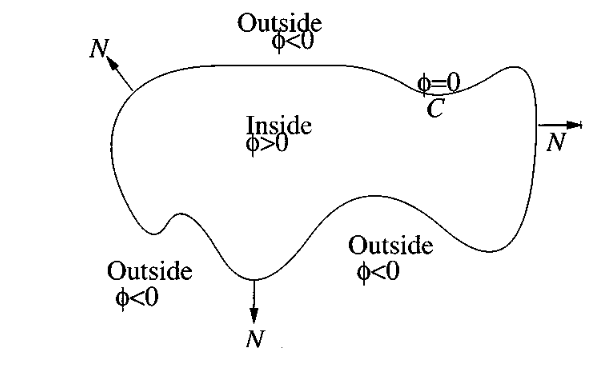
\includegraphics[height=0.5\textheight]{images/phi.png}
    \end{center}
    \vspace{-\baselineskip}
    \centering
    \justifying
    \scriptsize Illustration for the relationship between $C$ and $\phi$; Curve $C = \{ (x, y) : \phi(x, y) = 0 \}$ propagating in normal direction \cite{ChanVese}.
\end{frame}

\begin{frame}{The Level-Set Formulation}
    \begin{itemize}
        \item On the other hand, we can define the \emph{Heaviside} function $H(z)$ and the \emph{Dirac delta} function $\delta_0(z)$ as:
    \end{itemize}
    \[
        H(z) = \begin{cases}
            0, & \text{if } z < 0    \\
            1, & \text{if } z \geq 0
        \end{cases}, \,
        \delta_0(z) = \frac{d}{dz} H(z) = \begin{cases}
            \infty, & \text{if } z = 0,    \\
            0,      & \text{if } z \neq 0.
        \end{cases}
    \]
    \centering
    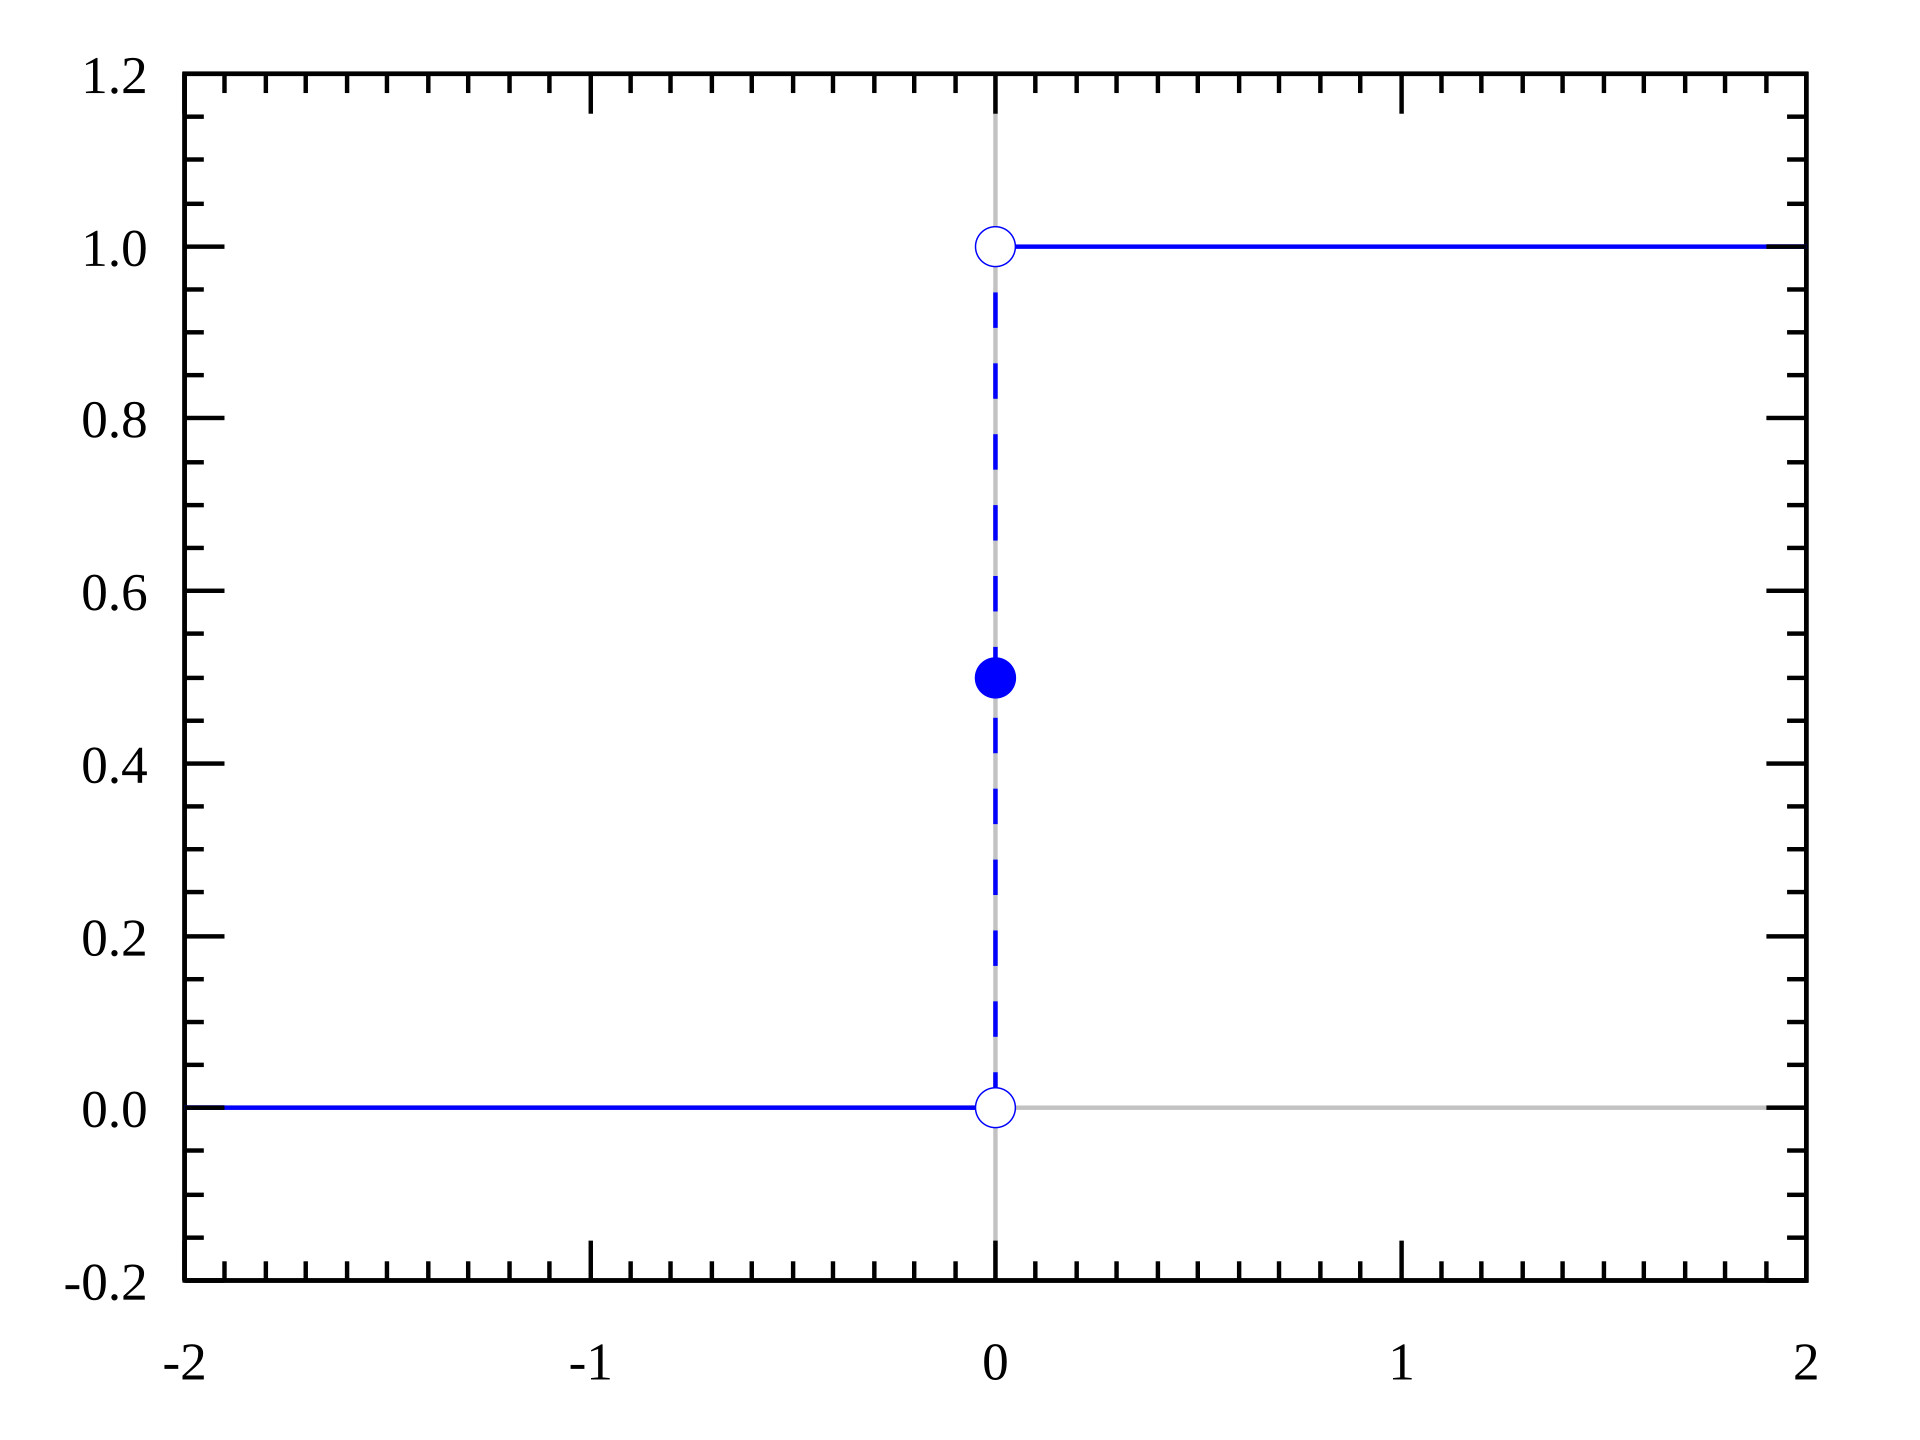
\includegraphics[width=0.45\textwidth]{images/heaviside.png}
    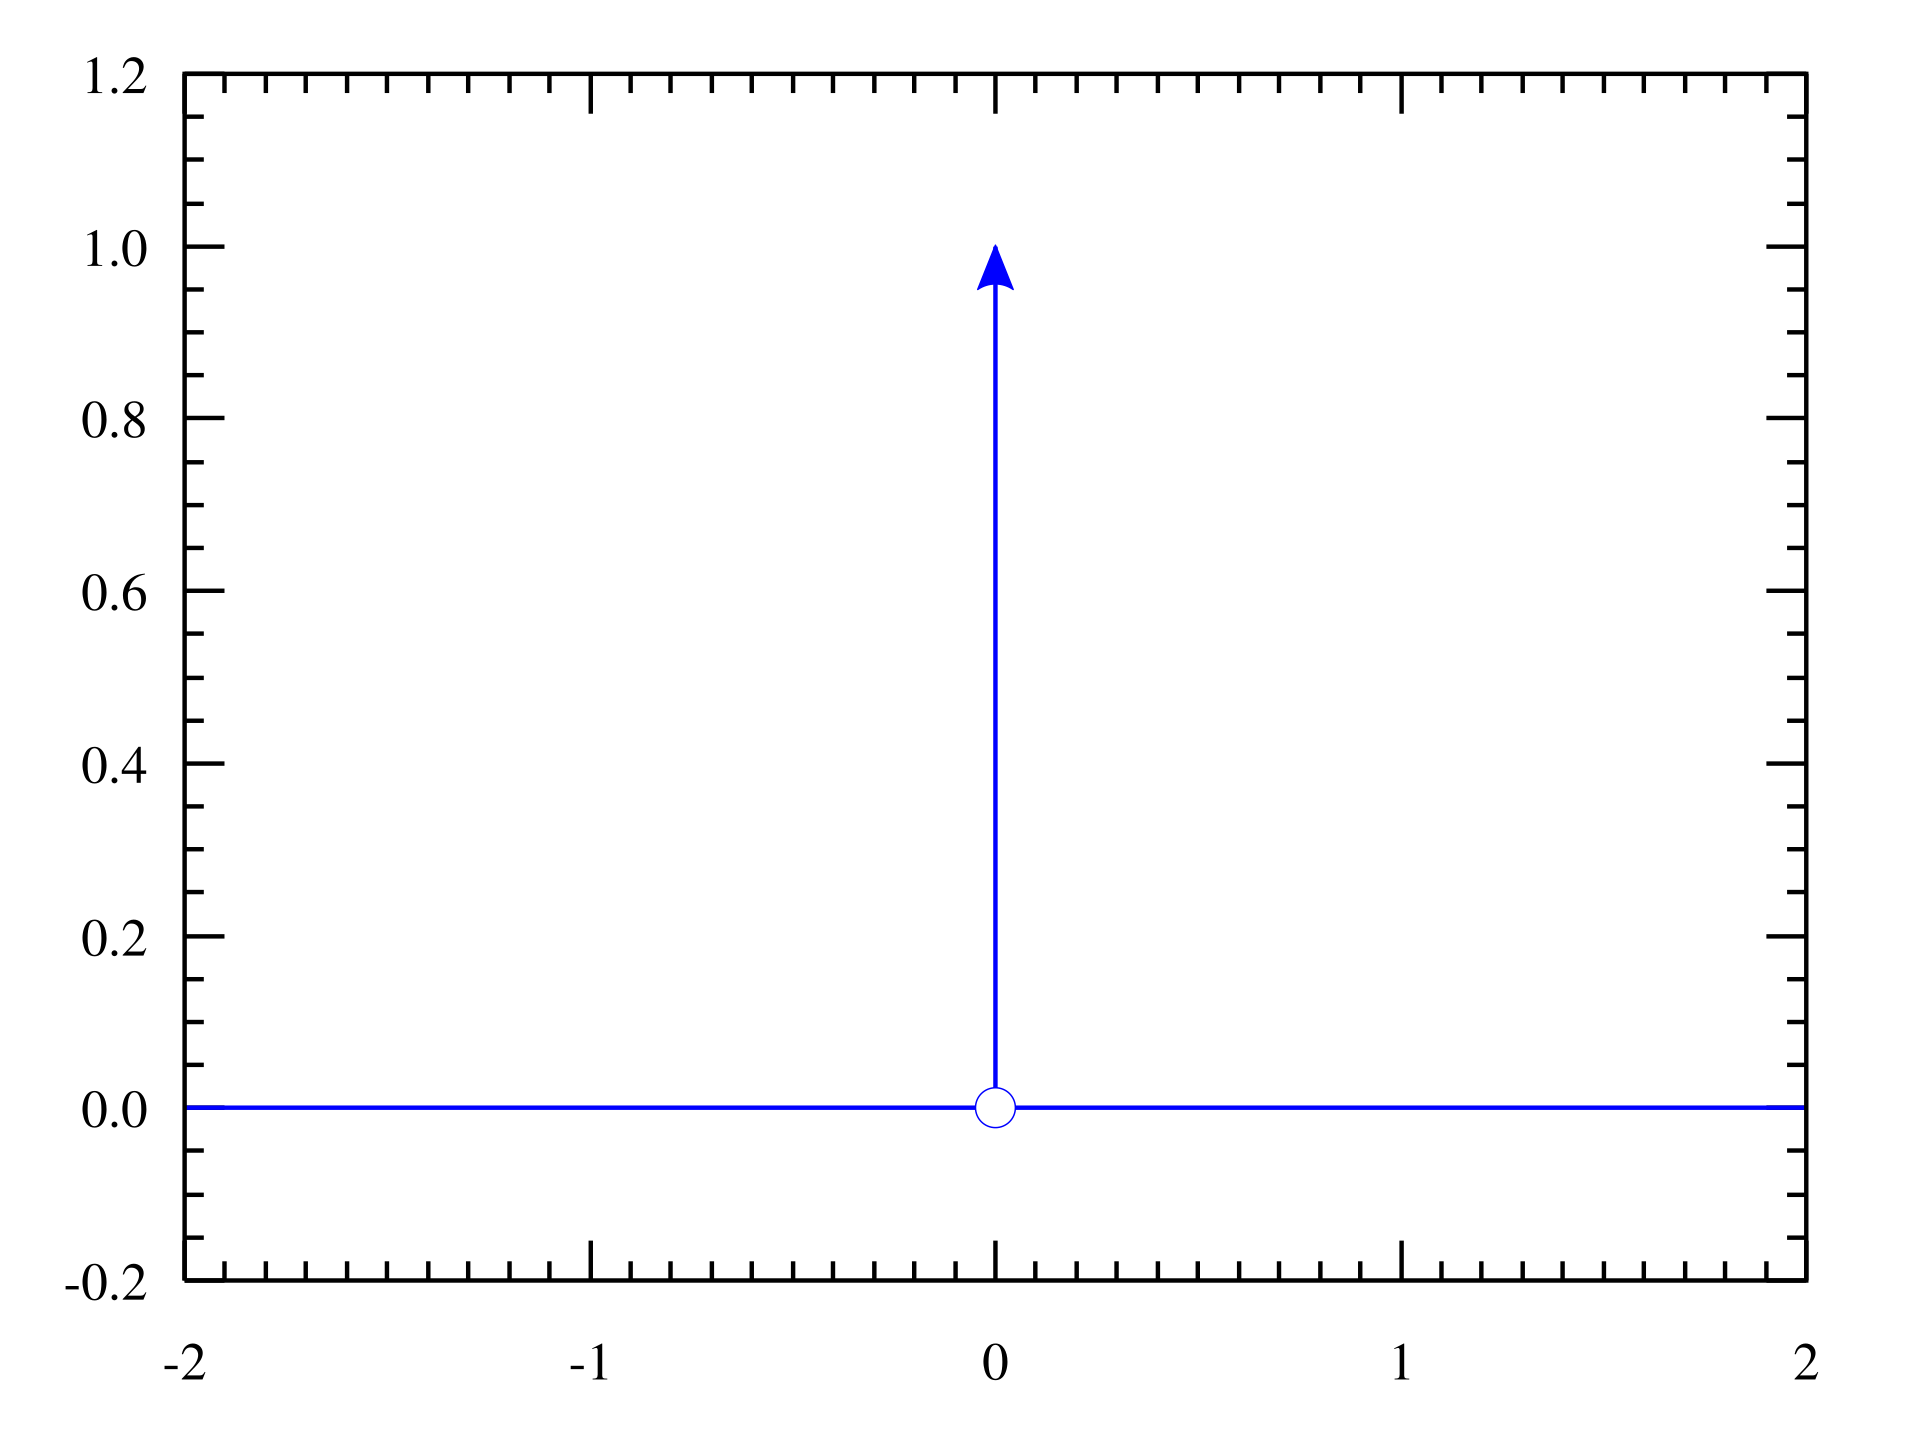
\includegraphics[width=0.45\textwidth]{images/dirac-delta.png}
    \vfill
    \scriptsize \textbf{Left:} Heaviside function $H(z)$ \cite{wiki:heaviside}, \textbf{Right:} its derivative $\delta_0(z)$, the one-dimensional Dirac measure \cite{wiki:dirac}.
\end{frame}

\begin{frame}{The Level-Set Formulation}
    \begin{itemize}
        \item With these definitions, it's clear that:
    \end{itemize}
    \begin{align*}
        \textrm{Length}\{\phi = 0\}  & = \int_{\Omega} |\nabla H(\phi(\bm{x}))| \, d\bm{x} = \int_{\Omega} \delta_0(\phi(\bm{x})) |\nabla \phi(\bm{x})| \, d\bm{x}, \\
        \textrm{Area}\{\phi \geq 0\} & = \int_{\Omega} H(\phi(\bm{x})) \, d\bm{x}
    \end{align*}
    \begin{center}
        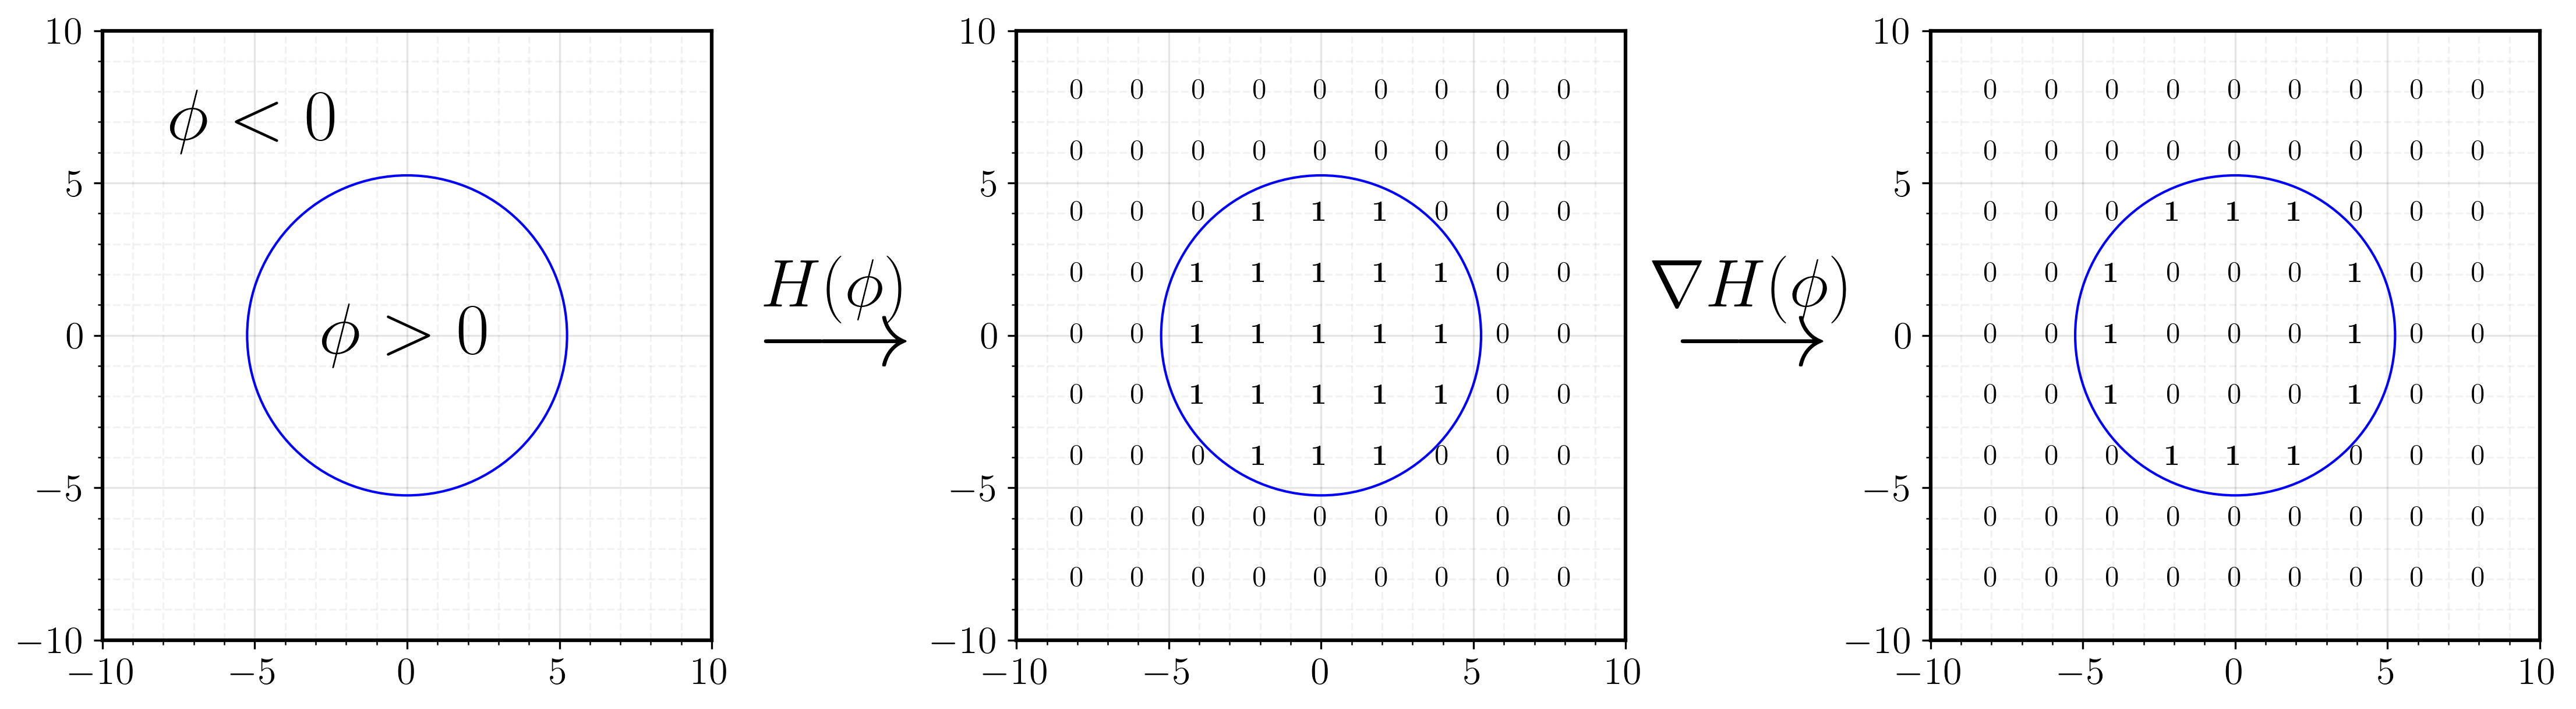
\includegraphics[width=\textwidth,keepaspectratio]{images/heaviside-and-phi-illustration.png}
        \vfill
        \scriptsize From \textbf{left} to \textbf{right}, the process of applying $H$ to $\phi$ and then taking the gradient.
    \end{center}
\end{frame}

\begin{frame}{The Level-Set Formulation}
    \begin{itemize}
        \item Thus, our energy functional $F(c_{in}, c_{out}, \phi)$ can be rewritten as:
              \begin{align*}
                  F(c_{in}, c_{out}, \phi)
                   & = \mu \underbrace{\color{purple}{\int_{\Omega} \delta(\phi(\bm{x})) |\nabla \phi(\bm{x})| \, d\bm{x}}}_{\textrm{\color{purple}{Length(C)}}} + \nu \underbrace{\color{purple}{\int_{\Omega} H(\phi(\bm{x})) \, d\bm{x}}}_{\textrm{\color{purple}{Area(inside(C))}}} \\
                   & \quad + \lambda_1 \underbrace{\color{blue}{\int_{\Omega} |u(\bm{x}) - c_{in}|^2 H(\phi(\bm{x})) \, d\bm{x}}}_{\text{$= $\color{blue}{$\int\limits_{\scriptscriptstyle inside(C)} \left| u(\bm{x}) - c_{in} \right|^2 d\bm{x}$}}}                                   \\
                   & \quad + \lambda_2 \underbrace{\color{red}{\int_{\Omega} |u(\bm{x}) - c_{out}|^2 (1 - H(\phi(\bm{x}))) \, d\bm{x}}}_{\text{$= $\color{red}{$\int\limits_{\scriptscriptstyle outside(C)} \left| u(\bm{x}) - c_{out} \right|^2 d\bm{x}$}}}                            \\
              \end{align*}
    \end{itemize}
\end{frame}

\begin{frame}{The Level-Set Formulation}
    \begin{itemize}
        \item In practice, $H$ and $\delta_0$ are approximated by \emph{continuous functions} $H_{\epsilon}$ and $\delta_{\epsilon}$, respectively, such that $H_\epsilon$ is at least $C^2(\bar{\Omega})$ and $\lim\limits_{\epsilon \to 0} H_{\epsilon}(z) = H(z)$ and $\lim\limits_{\epsilon \to 0} \delta_{\epsilon}(z) = \delta_0(z)$.
        \item \textbf{Chan and Vese (2001)} tried a $C^2(\bar{\Omega})$ regularization $H_{1, \epsilon}$ proposed in \cite{Zhao1996} and introduced a $C^\infty(\bar{\Omega})$ regularization $H_{2, \epsilon}$, defined as:
    \end{itemize}
    \[
        H_{1, \epsilon}(z) =
        \begin{cases}
            1                                                                                                            & \text{if } z > \epsilon      \\
            0                                                                                                            & \text{if } z < -\epsilon     \\
            \frac{1}{2} \left[ 1 + \frac{z}{\epsilon} + \frac{1}{\pi} \sin \left( \frac{\pi z}{\epsilon} \right) \right] & \text{if } |z| \leq \epsilon
        \end{cases}
    \]
    \[
        H_{2, \epsilon}(z) = \frac{1}{2} \left( 1 + \frac{2}{\pi} \arctan \left( \frac{z}{\epsilon} \right) \right)
    \]
\end{frame}

\begin{frame}{The Level-Set Formulation}
    \begin{center}
        \makebox[\textwidth][c]{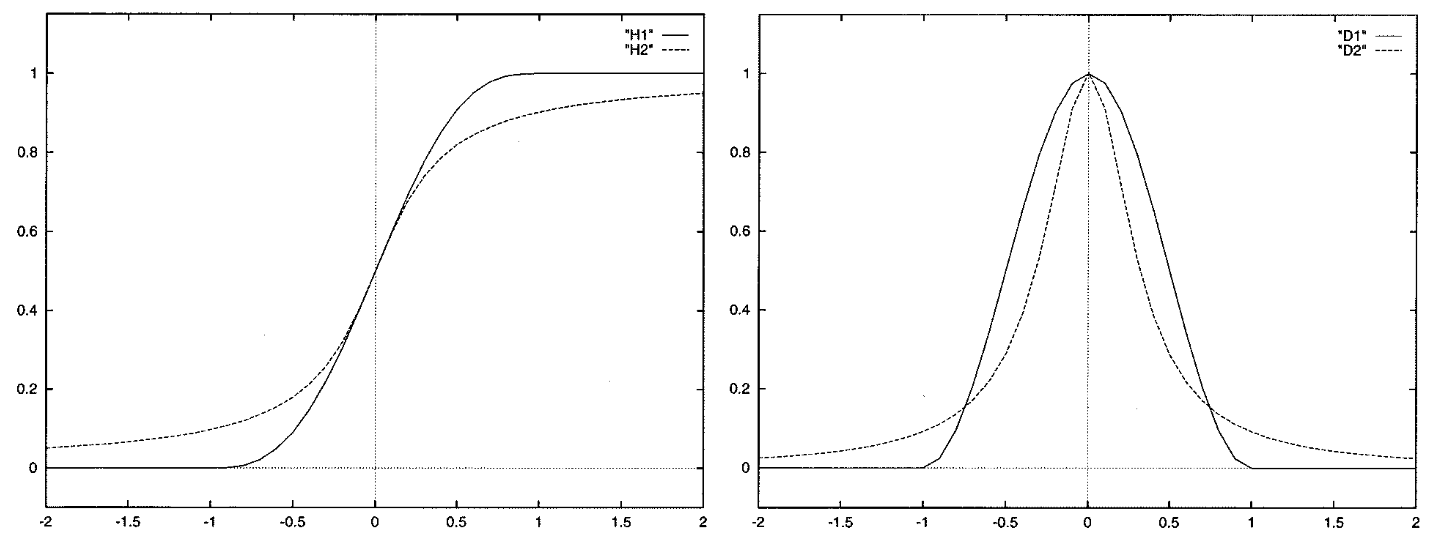
\includegraphics[width=1.1\textwidth]{images/heaviside-regularized.png}}
        \vfill
        \scriptsize Two different regularizations of the (left) heaviside function $H$ and (right) delta function $\delta_0$ \cite{ChanVese}.
    \end{center}
\end{frame}


\begin{frame}{The Level-Set Formulation}
    \begin{itemize}
        \item Finally, our \emph{regularized} energy functional $F_\epsilon(c_{in}, c_{out}, \phi)$ is given by:
    \end{itemize}
    \begin{align*}
        F(c_{in}, c_{out}, \phi)
         & = \mu \int_{\Omega} \delta_\epsilon(\phi(\bm{x})) |\nabla \phi(\bm{x})| \, d\bm{x} + \nu \int_{\Omega} H_\epsilon(\phi(\bm{x})) \, d\bm{x} \\
         & \quad + \lambda_1 \int_{\Omega} |u(\bm{x}) - c_{in}|^2 H_\epsilon(\phi(\bm{x})) \, d\bm{x}                                        \\
         & \quad + \lambda_2 \int_{\Omega} |u(\bm{x}) - c_{out}|^2 (1 - H_\epsilon(\phi(\bm{x}))) \, d\bm{x}                                 \\
    \end{align*}
\end{frame}
\subsection{Energy Minimization \& Discretization}

\begin{frame}{Euler-Lagrange Equation}
    \begin{itemize}
        \item Keeping $c_{in}$ and $c_{out}$ fixed, and minimizing $F_{\epsilon}$ with respect to $\phi$, we deduce the associated \emph{Euler--Lagrange} equation for $\phi$:
    \end{itemize}
    \[
        \begin{cases}
            F_\phi     & = \nu \delta_\epsilon(\phi) + \lambda_1 |u - c_{in}|^2 \delta_\epsilon(\phi) - \lambda_2 |u - c_{out}|^2 \delta_\epsilon(\phi), \\
            F_{\phi_x} & = 2 \mu \delta_\epsilon(\phi) \phi_x,                                                                                           \\
            F_{\phi_y} & = 2 \mu \delta_\epsilon(\phi) \phi_y                                                                                            \\
        \end{cases}
    \]
    \vspace{-0.5\baselineskip}
    \begin{alertblock}{Recall that...}
        The \bfit{Euler--Lagrange equation} for an energy functional of the form $E(\phi) = \int_{\Omega} F(x, y, \phi, \phi_x, \phi_y) \, d\bm{x}$ is
        $
            F_\phi - \partial_x F_{\phi_x} - \partial_y F_{\phi_y} = 0
        $
        with \textit{natural boundary conditions}
        $
            \bm{n}^\top \left( \begin{array}{c}
                    F_{\phi_x} \\
                    F_{\phi_y}
                \end{array} \right) = 0
        $
        where $\bm{n}$ denotes a normal vector to the image boundary $\partial \Omega$.
    \end{alertblock}
\end{frame}


\begin{frame}{Euler-Lagrange Equation}
    \begin{itemize}
        \item Thus, for $t \geq 0$, we get:
    \end{itemize}
    \begin{align*}
        \frac{\partial \phi}{\partial t} & = \delta_{\epsilon}(\phi) \left[ \mu \, \textrm{div} \left( \frac{\nabla \phi}{|\nabla \phi|} \right) - \nu - \lambda_1 (u - c_{in})^2 + \lambda_2 (u - c_{out})^2 \right] \\
                                         & = 0 \quad \textrm{in} \quad (0, \infty) \times \Omega
    \end{align*}
    \vspace{-1.5\baselineskip}
    \begin{itemize}
        \item With initial contour $\phi(0, x, y) = \phi_0(x, y) \, \, \textrm{in} \, \, \Omega$ and boundary condition:
    \end{itemize}
    \[
        \frac{\delta_{\epsilon}(\phi)}{|\nabla \phi|} \frac{\partial \phi}{\partial \vec{n}} = 0 \quad \textrm{on} \quad \partial \Omega
    \]
    \vspace{-0.5\baselineskip}
    \begin{itemize}
        \item[] where $\vec{n}$ denotes the exterior normal to the boundary $\partial \Omega$, and $\partial \phi / \partial \vec{n}$ denotes the normal derivative of $\phi$ at the boundary.
    \end{itemize}
\end{frame}

\begin{frame}{Discretization}
    \begin{itemize}
        \item To discretize this equation in $\phi$, \textbf{Chan and Vese(2001)} used a \emph{finite differences implicit scheme}.
    \end{itemize}
    \begin{block}{Usual Notations in Finite Differences}
        \begin{itemize}
            \item Let $h$ be \textbf{space step}; $\Delta t$, \textbf{time step}, and $(x_i, y_j) = (ih, jh)$ be the grid points, for $1 \leq i, j \leq M$.
            \item Let $\phi_{i,j}^n = \phi(n \Delta t, x_i, y_j) \approx \phi(t, x, y)$, with $n \geq 0$, $\phi^0 = \phi_0$.
            \item The finite differences are:
        \end{itemize}
        \[
            \begin{aligned}
                \Delta_-^x \phi_{i,j} & = \phi_{i,j} - \phi_{i-1,j}, \quad \Delta_+^x \phi_{i,j} & = \phi_{i+1,j} - \phi_{i,j}, \\
                \Delta_-^y \phi_{i,j} & = \phi_{i,j} - \phi_{i,j-1}, \quad \Delta_+^y \phi_{i,j} & = \phi_{i,j+1} - \phi_{i,j}
            \end{aligned}
        \]
    \end{block}
\end{frame}

\begin{frame}{Discretization}
    \begin{itemize}
        \item The following discretization and linearization of the PDE is used by \textbf{Chan and Vese (2001)}:
    \end{itemize}
    \small
    \begin{align*}
        \frac{\phi_{i,j}^{n+1} - \phi_{i,j}^n}{\Delta t}
         & = \delta_h(\phi_{i,j}^n) \Bigg[ \frac{\mu}{h^2} \Delta_-^x                                                                         \\
         & \quad \cdot \left(
        \frac{\Delta_+^x \phi_{i,j}^{n+1}}{\sqrt{(\Delta_+^x \phi_{i,j}^n)^2 / (h^2) + (\phi_{i,j+1}^n - \phi_{i,j-1}^n)^2 / (2h)^2}} \right) \\
         & \quad + \frac{\mu}{h^2} \Delta_-^y \cdot \left(
        \frac{\Delta_+^y \phi_{i,j}^{n+1}}{\sqrt{(\phi_{i+1,j}^n - \phi_{i-1,j}^n)^2 / (2h)^2 + (\Delta_+^y \phi_{i,j}^n)^2 / (h^2)}} \right) \\
         & \quad - \nu - \lambda_1 (u_{i,j} - c_1(\phi^n))^2 + \lambda_2 (u_{i,j} - c_2(\phi^n))^2 \Bigg]
    \end{align*}
\end{frame}

\begin{frame}{Principal Steps of the Algorithm}
    \small
    \begin{algorithm}[H]
        \caption{The Level-Set Algorithm}
        \SetAlgoLined
        \KwIn{Initial level-set function $\phi_0$, $n = 0$}
        \KwResult{Updated level-set function $\phi$}
        \Begin{
            Initialize $\phi^0$ by $\phi_0$, $n = 0\;$ \\
            \While{the solution is not stationary}{
                Compute $c_{in}(\phi^n)$ and $c_{out}(\phi^n)$ based on the current state;
                Solve the PDE in $\phi$ from the previous eq., to obtain $\phi^{n+1}$\;
                Check whether the solution is stationary\;
                \If{not stationary}{
                    $n = n + 1$\;
                }
            }
        }
    \end{algorithm}
\end{frame}

\section{Results}

\begin{frame}{Parameter Selection}
    \begin{itemize}
        \item \( \lambda_1 = \lambda_2 = 1 \), \( \nu = 0 \), \( h = 1 \) (the step space), \( \Delta t = 0.1 \) (the time step).
        \item \( H_{2,\epsilon} \) and \( \delta_{2,\epsilon} \) were used with (\( \epsilon = h = 1 \)), in order to automatically detect \emph{interior contours}, and to ensure the computation of a \emph{global minimizer}.
        \item $\mu$ is \emph{experiment-dependent}:
              \begin{itemize}
                  \item Detect as many objects as possible $\Longrightarrow \text{small} \, \, \mu$.
                  \item Detect only larger objects $\Longrightarrow \text{large} \, \, \mu$.
              \end{itemize}
    \end{itemize}
\end{frame}


\begin{frame}{Comparison between $H_{1, \epsilon}$ and $H_{2, \epsilon}$ regularizations}
    \hypertarget{SmallerDiracDelta}{}
    \begin{itemize}
        \item The energy functional $F_\epsilon$ is \emph{non-convex}, allowing therefore many local minima.
        \item With \( H_{1,\epsilon} \) and \( \delta_{1,\epsilon} \Longrightarrow \) local minimizer of the energy.
        \item With \( H_{2,\epsilon} \) and \( \delta_{2,\epsilon} \Longrightarrow \) global minimizer of the energy.
    \end{itemize}
    \vfill
    \centering
    \hyperlink{LargerDiracDelta}{%
        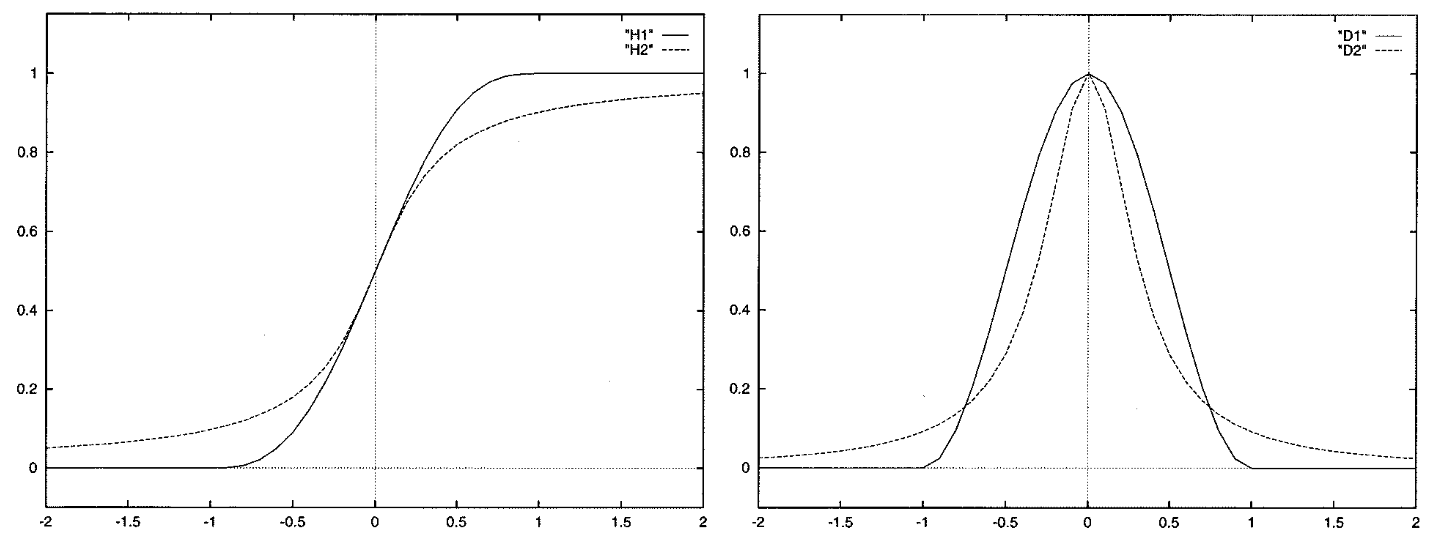
\includegraphics[height=0.4\textheight]{images/heaviside-regularized.png}}
    \vfill
    \scriptsize Two different regularizations of the (left) heaviside function $H$ and (right) delta function $\delta_0$ \cite{ChanVese}
\end{frame}

\begin{frame}{Results}
    \begin{center}
        \makebox[\textwidth][c]{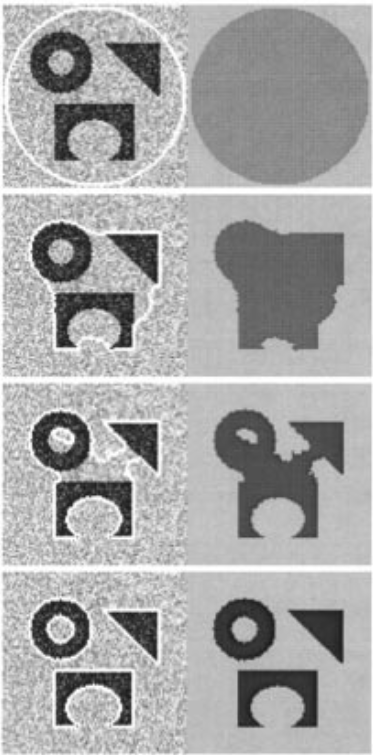
\includegraphics[width=1.2\textwidth,height=1.2\textheight,origin=c,angle=90,keepaspectratio]{images/results-noisy-detection.png}}
    \end{center}
    \vspace{-5.5\baselineskip}
    \justifying
    \scriptsize Detection of different objects from a noisy image, with various shapes and with an interior contour. \textbf{Left:} \( u \) and the contour. \textbf{Right:} the piecewise-constant approximation of \( u \). Size = \( 100 \times 100 \), \( \phi_0(x, y) = -\sqrt{(x - 50.5)^2 + (y - 50.5)^2} + 48.5 \), \( \mu = 0.1 \times 255^2 \), no reinitialization, cpu = 4.60 s \cite{ChanVese}.
    \note{
        \begin{itemize}
            \item The model works on a noisy synthetic image, with various shapes and an interior contour, which is automatically detected, without considering a second initial curve.
            \item Due to the level set implementation, the model allows automatical change of topololgy.
        \end{itemize}
    }
\end{frame}

\begin{frame}{Results}
    \begin{center}
        \makebox[\textwidth][c]{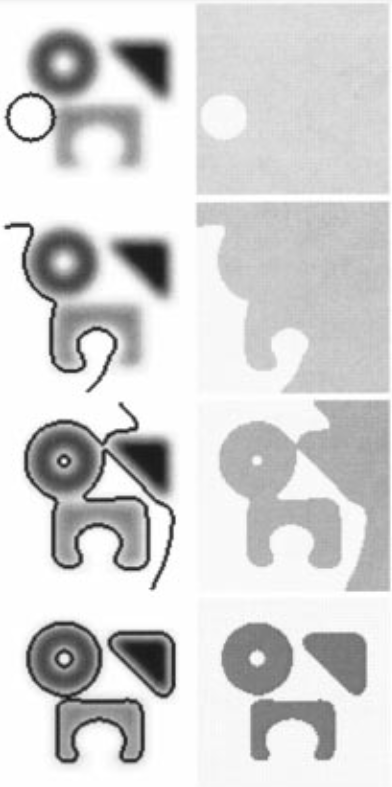
\includegraphics[width=1.2\textwidth,height=1.2\textheight,origin=c,angle=90,keepaspectratio]{images/results-blurry-detection.png}}
    \end{center}
    \vspace{-5.5\baselineskip}
    \justifying
    \scriptsize Detection of three blurred objects of distinct intensities. Size = \(100 \times 100\), \(\phi_0(x, y) = -\sqrt{(x - 15)^2 + (y - 60)^2} + 12\), \(\mu = 0.01 \cdot 255^2\), no reinitialization, cpu = 48.67 s \cite{ChanVese}.
    \note{
        \begin{itemize}
            \item The model can detect different objects of different intensities, and with blurred boundaries.
            \item The interior contour of the torus is automatically detected.
            \item This is also due to the fact that the velocity has a global dependence, and the curve is automatically attracted toward the objects.
            \item The initial curve does not necessarily surround the objects.
        \end{itemize}
    }
\end{frame}

\begin{frame}{Results}
    \vspace{-\baselineskip}
    \begin{center}
        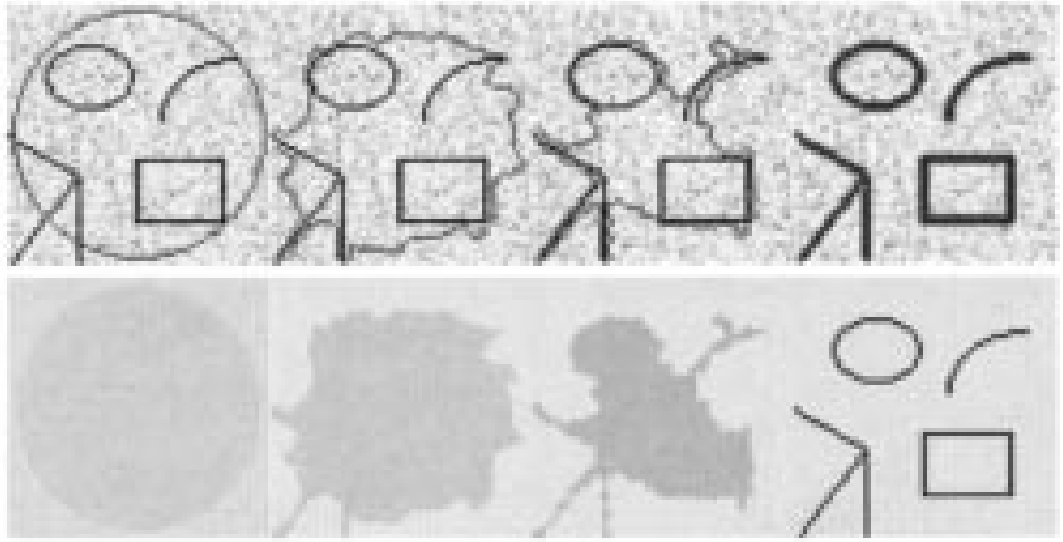
\includegraphics[width=\textwidth,height=0.8\textheight,keepaspectratio]{images/results-lines.png}
    \end{center}
    \vfill
    \vspace{-\baselineskip}
    \justifying
    \scriptsize Detection of lines and curves not necessarily closed. Size = \(64 \times 64\), \(\phi_0(x, y) = -\sqrt{(x - 32.5)^2 + (y - 32.5)^2} + 30\), \(\mu = 0.02 \cdot 255^2\), no reinitialization, cpu = 2.88 s \cite{ChanVese}.
    \note{
        \begin{itemize}
            \item The model can detect lines and curves (not necessarily closed) in a noisy image.
            \item The final level set function is zero on the curves and negative outside the curve.
        \end{itemize}
    }
\end{frame}

\begin{frame}{Results}
    \vspace{-\baselineskip}
    \begin{center}
        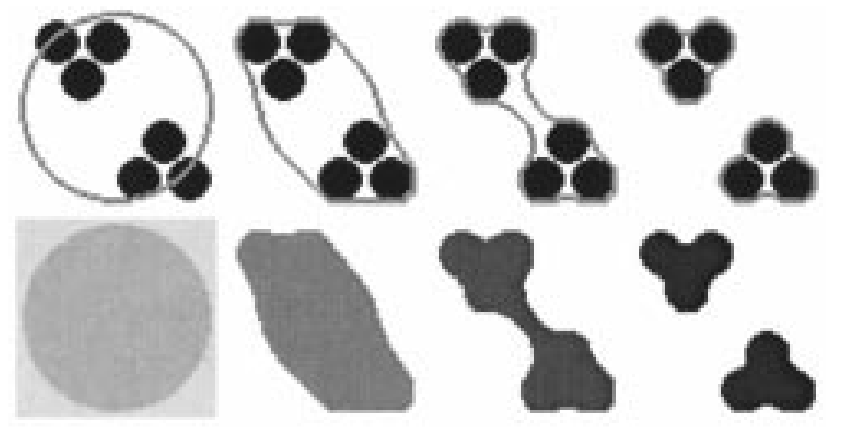
\includegraphics[width=\textwidth,height=0.8\textheight,keepaspectratio]{images/results-kanizsa.png}
    \end{center}
    \vfill
    \vspace{-\baselineskip}
    \justifying
    \scriptsize Grouping based on Kanizsa's ``proximity rule.'' Size = \(64 \times 64\), \\
    \(\phi_0(x, y) = -\sqrt{(x - 32.5)^2 + (y - 32.5)^2} + 30\), \(\mu = 2 \cdot 255^2\), no reinitialization, cpu = 5.76 s \cite{ChanVese}.
    \note{
        \begin{itemize}
            \item Illustrates the role of the length term, $mu$, as a scale parameter.
            \item Previous slides had $m$ small, therefore prioritizing segmentation of smaller objects and not groups of objects.
            \item If is small, then also smaller objects will be detected; if is larger, then only larger objects are detected, or objects formed by grouping.
            \item This slide shows it can detect objects defined by grouping according to Kanizsa's "proximity rule".
            \item Next slides show how the grouping is based on the chromatic resemblance or identity, among objects of the same shape.
        \end{itemize}
    }
\end{frame}

\begin{frame}{Results}
    \begin{center}
        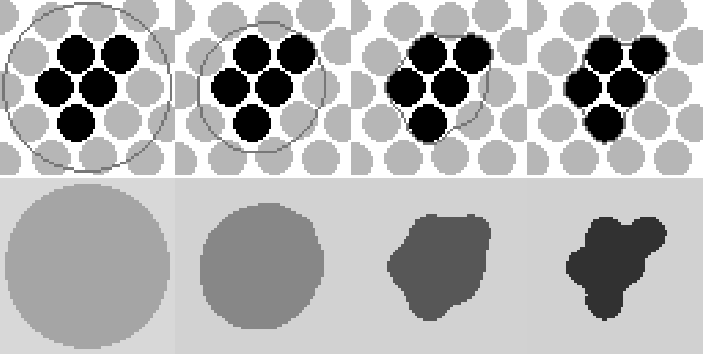
\includegraphics[width=0.95\textwidth,keepaspectratio]{images/results-grouping.png}
    \end{center}
    \scriptsize Grouping based on chromatic identity. Size: $64 \times 64$, $\phi_0(x, y) = -\sqrt{(x - 32.5)^2 + (y - 32.5)^2} + 30.5$, $\mu = 2 \cdot 255^2$, no reinitialization, cpu = 5.76 s. \cite{ChanVese}.
\end{frame}

\begin{frame}{Results}
    \begin{center}
        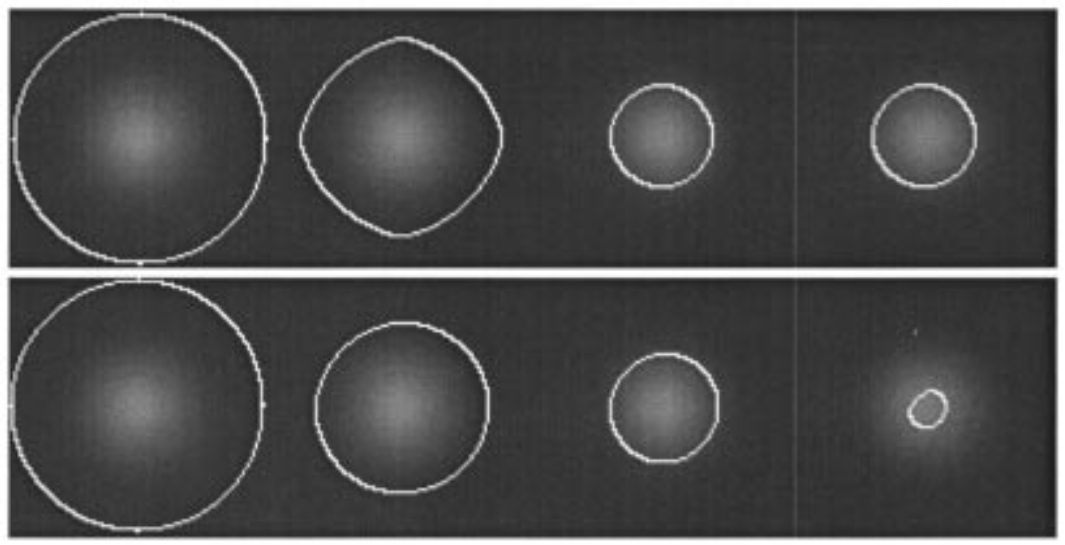
\includegraphics[width=0.95\textwidth,keepaspectratio]{images/results-smooth.png}
    \end{center}
    \vfill
    \vspace{-\baselineskip}
    \centering
    \justifying
    \scriptsize Object with smooth contour. \textbf{Top:} results using the \textbf{Chan--Vese model} without edge-function. \textbf{Bottom:} results using the classical model (2) with edge-function $g(|\nabla u|)$, by which the curve cannot detect the smooth boundary \cite{ChanVese}.
\end{frame}

\begin{frame}{Results}
    \begin{center}
        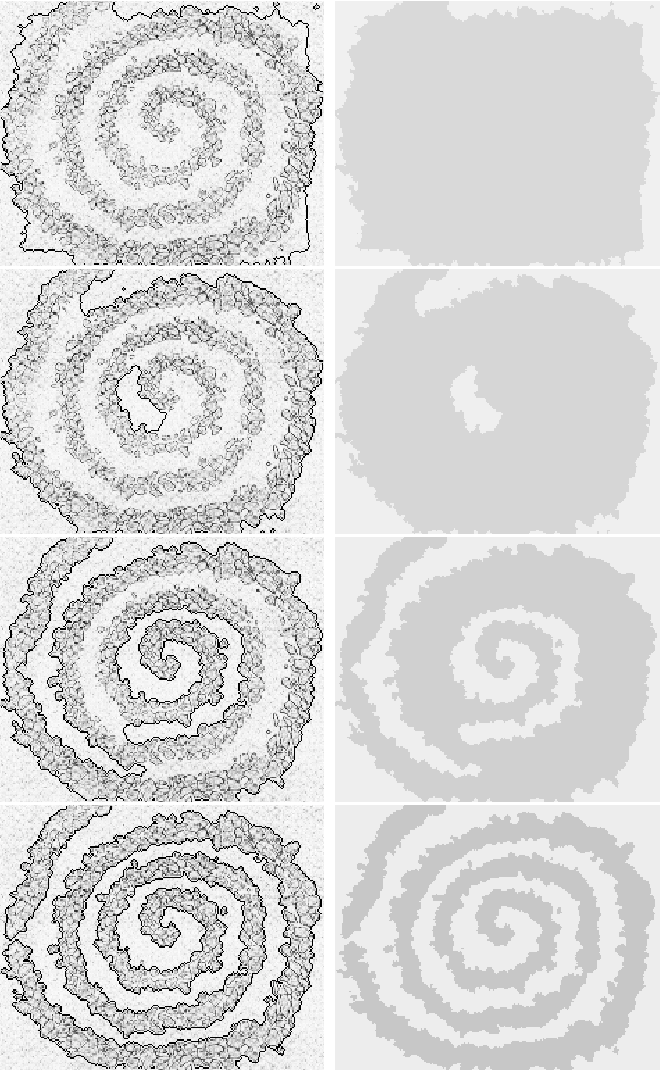
\includegraphics[angle=90,origin=c,height=0.9\textheight,keepaspectratio]{images/results-spiral.png}
    \end{center}
    \vspace{-4\baselineskip}
    \scriptsize Spiral from an art picture. Size = $234 \times 191$, $\mu = 0.0000033 \cdot 255^2$, five iterations of reinitialization, cpu = 108.85 s \cite{ChanVese}.
    \note{
        \begin{itemize}
            \item Art picture from the Los Angeles Times by Brian Forrest.
            \item For the length penalization, they used an exponent of 2 instead of 1.
            \item The initial curve is the boundary of the image. After a time, a curve in the middle of the image appears and expands until merges with the initial evolving curve.
        \end{itemize}
    }
\end{frame}

\begin{frame}{Advantages of the Model}
    \begin{itemize}
        \item The ability of detecting smooth boundaries.
        \item Scale adaptivity (with the parameter $\mu$).
        \item Automatic change of topology.
        \item Robustness with respect to noise.
        \item Flexibility in handling various image types, even without much parameter tuning.
    \end{itemize}
\end{frame}

\begin{frame}{Limitations of the Model}
    \begin{itemize}
        \item The \textbf{Chan--Vese (2001)} model is a specific case of the Mumford--Shah functional.
        \item There are objects which cannot be detected using the \emph{average intensity value} only.
    \end{itemize}
    \vfill
    \begin{minipage}{0.45\textwidth}
        \centering
        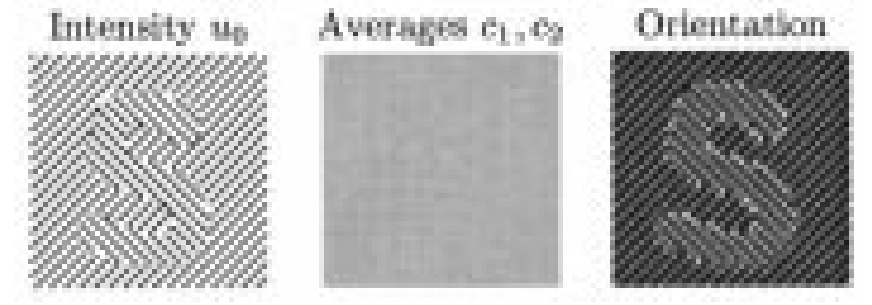
\includegraphics[width=\textwidth]{images/limitations-images.png}
    \end{minipage}
    \hfill
    \begin{minipage}{0.45\textwidth}
        \centering
        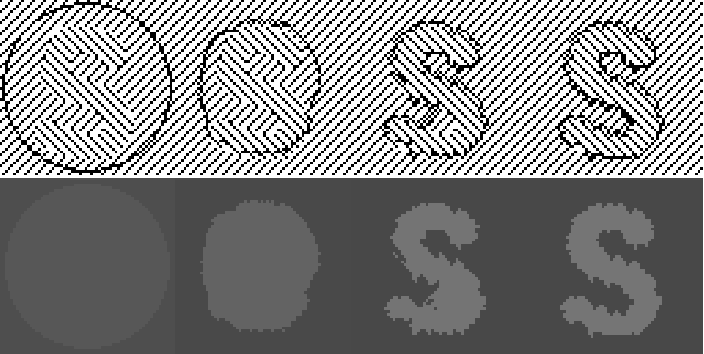
\includegraphics[width=\textwidth]{images/limitations.png}
    \end{minipage}
    \vfill
    \centering
    \justifying
    \scriptsize Grouping based on orientation identity. The original image $u$ (\textbf{leftmost}) is replaced by the orientation of the normal to the level curves of $u$. Size: $64 \times 64$, $\mu = 0.025 \cdot 255^2$, $\nu = 0.02 \cdot 255^2$, $\phi_0(x, y) = -\sqrt{(x - 32.5)^2 + (y - 32.5)^2} + 30$, five iterations of reinitialization, cpu = $10.25$ s \cite{ChanVese}.
\end{frame}

\section{Impact on Research}

\subsection{Real-World Applications}

\begin{frame}{Segmentation on Satellite Images}
    \begin{center}
        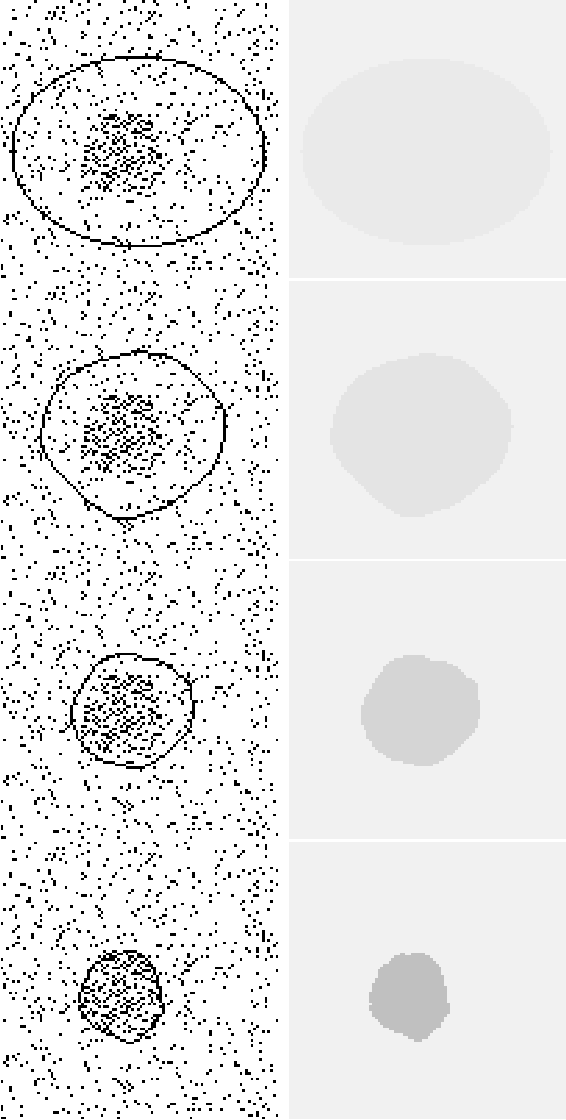
\includegraphics[angle=90,origin=c,height=0.9\textheight,keepaspectratio]{images/results-simulated-mine.png}
    \end{center}
    \vspace{-5\baselineskip}
    \scriptsize Detection of a simulated minefield, with contour without gradient.\\
    Size = $100 \times 100$, $\phi_0(x, y) = -\sqrt{(x - 50.5)^2 + (y - 50.5)^2} + 47$, $\mu = 0.2 \cdot 255^2$, no reinitialization, cpu = 144.81 s \cite{ChanVese}.
    \note{
        \begin{itemize}
            \item Different problem: detect features in spatial point processes in the presence of substantial cluster.
            \item Real-World Application: detection of minefields using reconnaissance aircraft images that identify many objects that are not mines. These problems are usually solved using statistical methods.
            \item This model can be used to detect objects or features with contours without gradient. This is not possible using classical snakes or active contours based on the gradient.
            \item Similar application is presented where the white points are Europe night-lights.
        \end{itemize}
    }
\end{frame}

\begin{frame}{Segmentation on Satellite Images}
    \begin{center}
        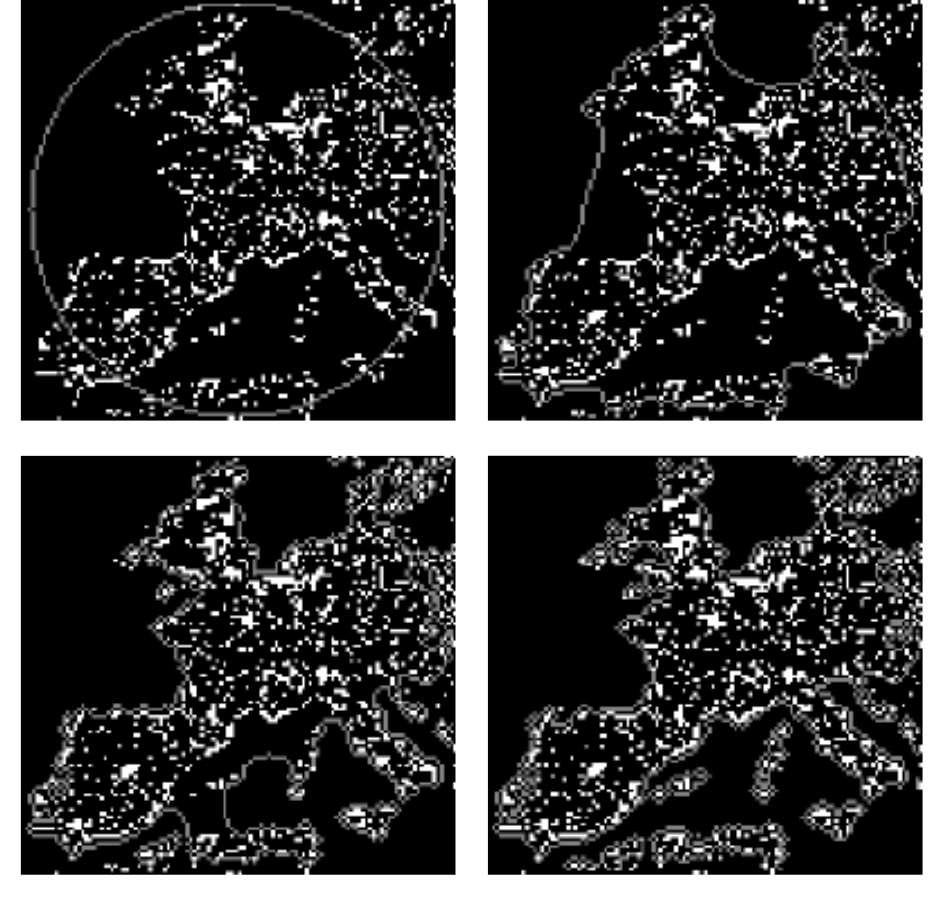
\includegraphics[height=0.75\textheight,keepaspectratio]{images/results-europe-light.png}
    \end{center}
    \vspace{-0.75\baselineskip}
    \scriptsize Europe night-lights. Size = $118 \times 113$, $\phi_0(x, y) = -\sqrt{(x - 59.)^2 + (y - 57.)^2} + 55$, $\mu = 0.05 \cdot 255^2$, five iterations of reinitialization, cpu = 32.74 s \cite{ChanVese}.
\end{frame}

\begin{frame}{Segmentation on Satellite Images}
    \begin{center}
        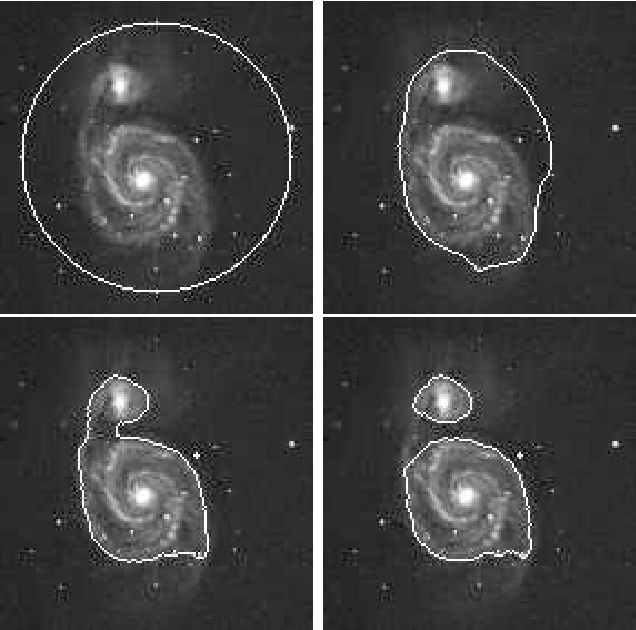
\includegraphics[height=0.75\textheight,keepaspectratio]{images/results-galaxy.png}
    \end{center}
    \vspace{-0.25\baselineskip}
    \centering
    \scriptsize Detection of the contours of a galaxy \cite{ChanVese}.
\end{frame}

\begin{frame}{Segmentation on Satellite Images}
    \begin{center}
        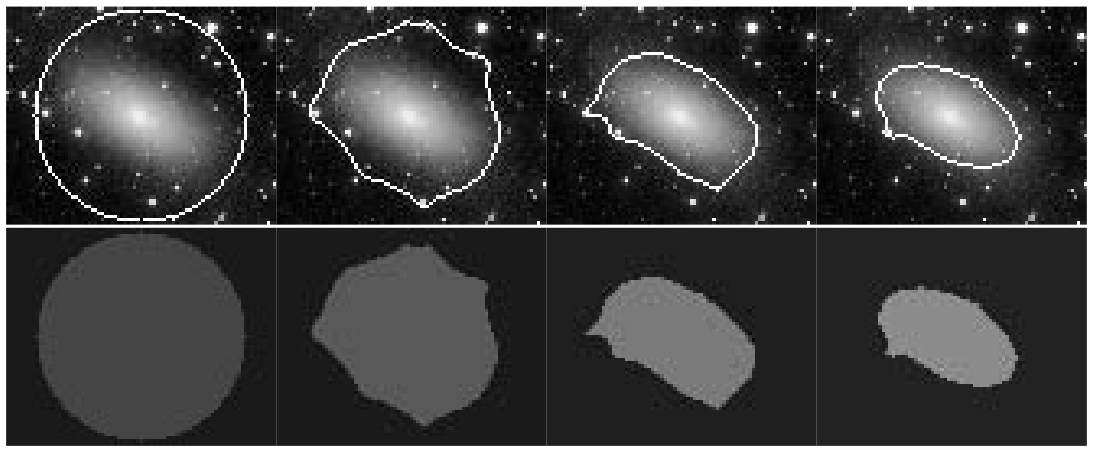
\includegraphics[width=\textwidth,keepaspectratio]{images/results-galaxy-2.png}
    \end{center}
    \vspace{-0.25\baselineskip}
    \centering
    \scriptsize Detection of a galaxy with very smooth boundaries \cite{ChanVese}.
\end{frame}

\begin{frame}{Segmentation on MRI Images}
    \begin{center}
        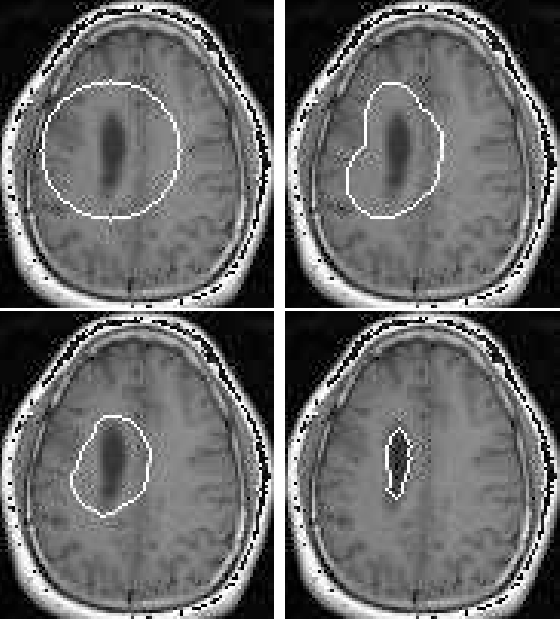
\includegraphics[height=0.8\textheight,keepaspectratio]{images/results-mri.png}
    \end{center}
    \vspace{-0.5\baselineskip}
    \centering
    \scriptsize Detection of a tumor in a MRI image \cite{ChanVese}.
\end{frame}

\begin{frame}{Implementations}
    \begin{itemize}
        \item Available as a segmentation method in \emph{scikit-image} (Python).
        \item Integrated as a \href{https://de.mathworks.com/matlabcentral/fileexchange/23445-chan-vese-active-contours-without-edges}{\color{blue}{Plugin in MATLAB by Yue Wu}}.
        \item Integrated in \href{https://itk.org/}{\color{blue}{Insight Toolkit (ITK)}}, an open-source, cross-platform library for image analysis.
    \end{itemize}
    \vfill
    \begin{minipage}{0.32\textwidth}
        \centering
        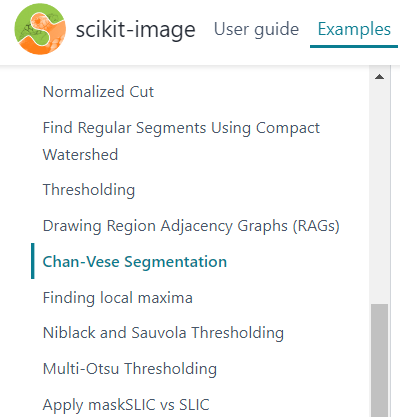
\includegraphics[width=\textwidth]{images/implementations-scikit-learn.png}
    \end{minipage}
    \hfill
    \begin{minipage}{0.32\textwidth}
        \centering
        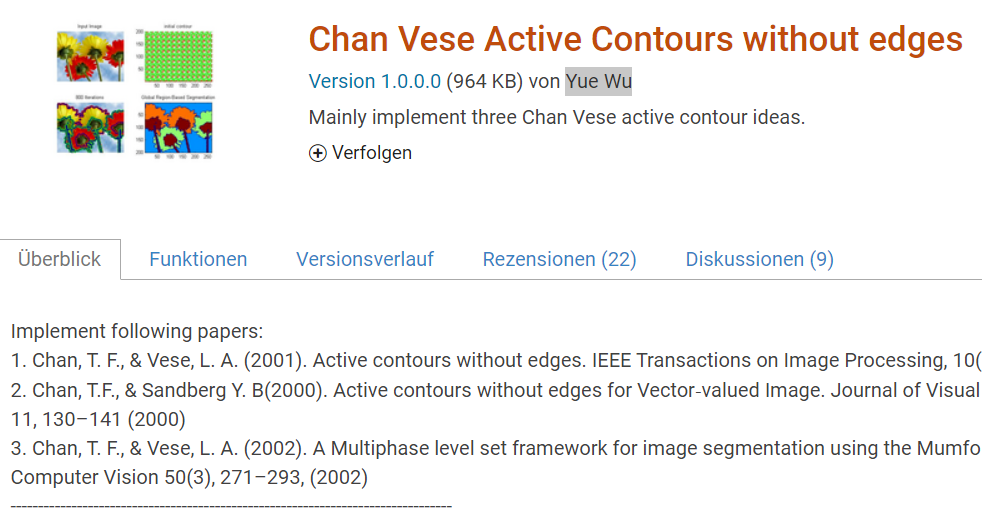
\includegraphics[width=\textwidth]{images/implementations-matlab.png}
    \end{minipage}
    \hfill
    \begin{minipage}{0.32\textwidth}
        \centering
        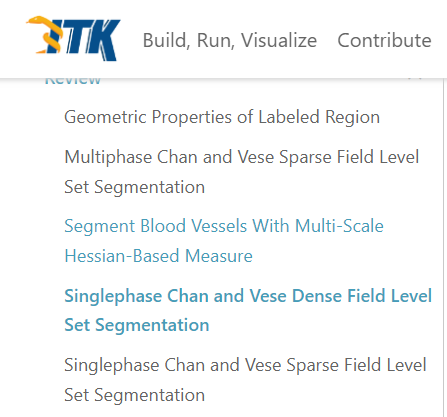
\includegraphics[width=\textwidth]{images/implementations-itk.png}
    \end{minipage}
    \vfill
    \centering
    \scriptsize Some widely-spread implementations of the \textbf{Chan--Vese model} in software.
\end{frame}

\subsection{Current Approaches}

\begin{frame}{Derivative Works}
    \scriptsize
    \begin{center}
        % Define row colors
        \rowcolors{1}{gray!25}{white} % Alternate row colors
        \begin{tabularx}{\textwidth}{>{\columncolor{gray!25}}X >{\columncolor{gray!25}}l >{\columncolor{gray!25}}c >{\columncolor{gray!25}}c}
            \toprule
            \textbf{Title}                                                                                          & \textbf{Last Author} & \textbf{Year} & \textbf{Citations} \\
            \midrule
            Level Set Method in Medical Imaging Segmentation                                                        & J. Suri              & 2019          & 12                 \\
            Efficient and robust segmentation and correction model for medical images                               & W. Jia               & 2018          & 3                  \\
            A two-stage image segmentation via global and local region active contours                              & Yugang Wang          & 2016          & 49                 \\
            Active contours driven by local likelihood image fitting energy for image segmentation                  & Qiang Chen           & 2015          & 94                 \\
            Robust image segmentation using local robust statistics and correntropy-based K-means clustering        & Li Zeng              & 2015          & 23                 \\
            An active contour model and its algorithms with local and global Gaussian distribution fitting energies & Yilun Wang           & 2014          & 86                 \\
            An efficient operator splitting method for local region Chan-Vese model                                 & Jun Liu              & 2013          & 2                  \\
            \bottomrule
        \end{tabularx}
    \end{center}
    \vfill
    \begin{center}
        \scriptsize Courtesy of \href{https://www.connectedpapers.com/}{@ConnectedPapers}, this table available \href{https://www.connectedpapers.com/main/3bdcc6c663112ab10ffb5b5e875f8e2660cd5001/Active-contours-without-edges/derivative}{here}.
    \end{center}
\end{frame}

\begin{frame}{Extensions of the Chan-Vese Model}
    \begin{itemize}
        \item Modifications of the \textbf{Chan--Vese model} include \cite{Pascal2023}:
              \begin{itemize}
                  \item More sophisticated features than the grey value
                        \begin{itemize}
                            \item Colour channels, texture features, optic flow fields, ...
                        \end{itemize}
                  \item Additional statistical characterizations of a region
                        \begin{itemize}
                            \item Not only mean, but also standard deviation, ...
                        \end{itemize}
                  \item A-priori knowledge, using a statistical characterization of the shapes to be expected
              \end{itemize}
        \item Can yield excellent segmentation results
    \end{itemize}
\end{frame}

\begin{frame}{Extensions of the Chan--Vese Model}
    \begin{center}
        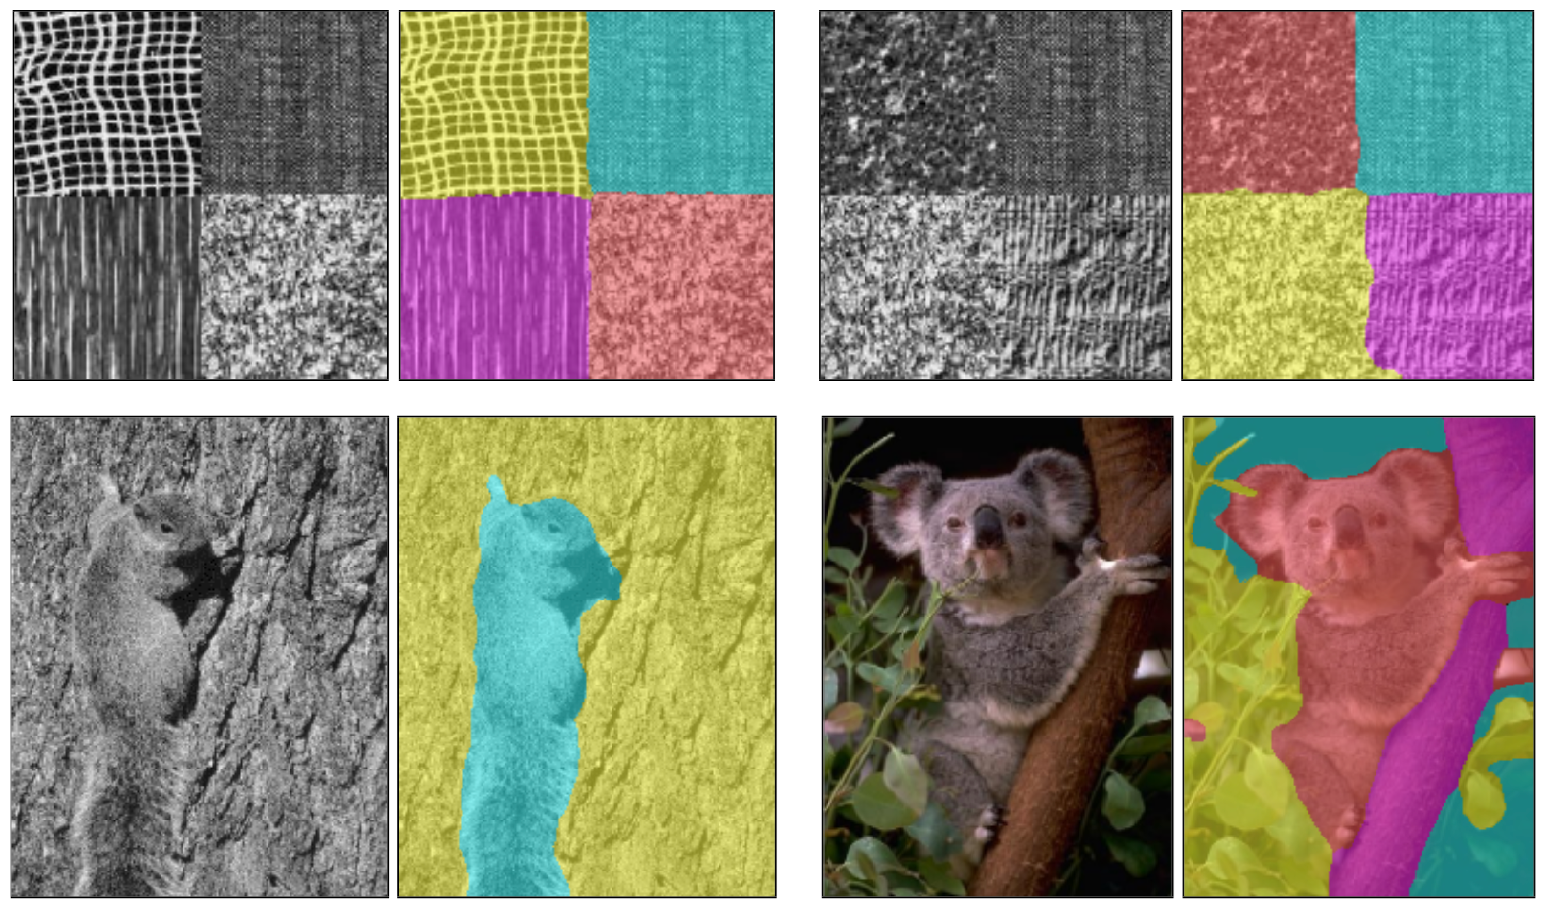
\includegraphics[height=0.5\textwidth]{images/honorable-mentions-1-2-combined.png}
    \end{center}
    \vspace{-0.5\baselineskip}
    \centering
    \justifying
    \scriptsize \textbf{Top:} Segmentation of two artificial texture images: In both cases 4 regions were detected. \textbf{Bottom left:} Segmentation of a squirrel image: 2 regions have been detected. \textbf{Bottom right:} Segmentation of a koala image (colour): 4 regions have been detected.
    Author: T. Brox (2004) \cite{Brox2004}.
\end{frame}

\begin{frame}{Extensions of the Chan--Vese Model}
    \begin{center}
        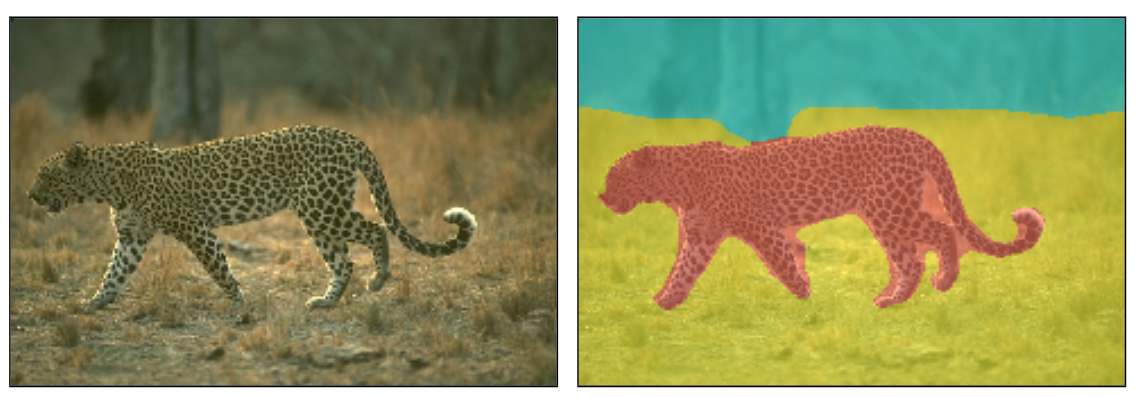
\includegraphics[height=0.25\textwidth]{images/honorable-mentions-3.png}\\
        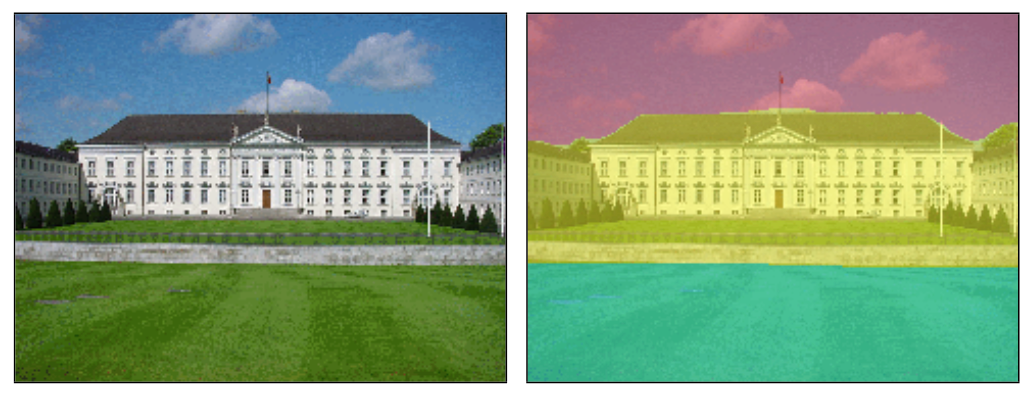
\includegraphics[height=0.25\textwidth]{images/honorable-mentions-4.png}
    \end{center}
    \vspace{-0.5\baselineskip}
    \centering
    \justifying
    \scriptsize \textbf{Top:} Segmentation of a leopard image (colour): 3 regions have been detected. \textbf{Bottom:} Segmentation of a castle image (colour): 3 regions have been detected.
    Author: T. Brox (2004) \cite{Brox2004}.
\end{frame}

\begin{frame}{Extensions of the Chan--Vese Model}
    \begin{center}
        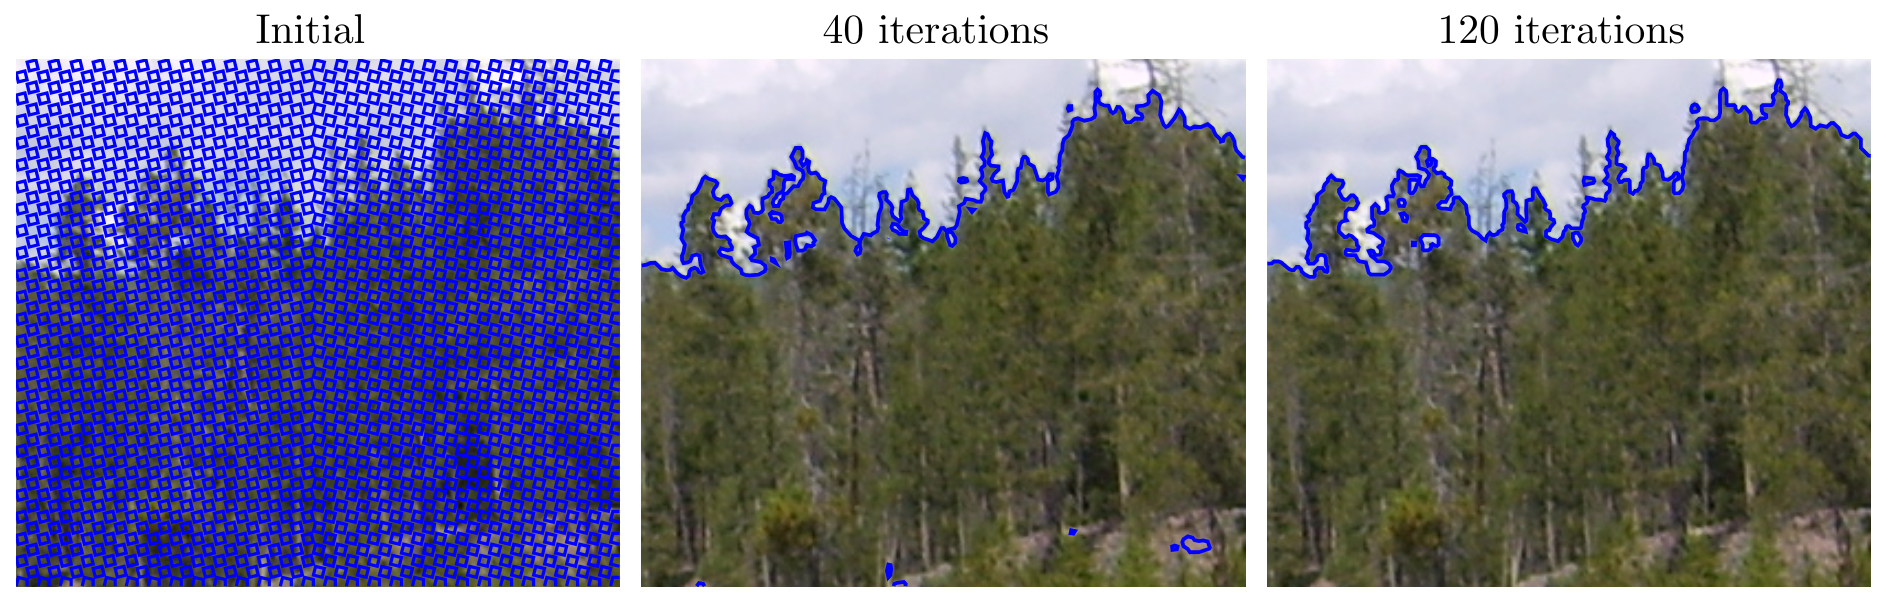
\includegraphics[width=\textwidth]{images/honorable-mentions-7.png}
    \end{center}
    \vspace{-0.5\baselineskip}
    \centering
    \justifying
    \scriptsize The \textbf{Chan--Sandberg--Vese (2000)} method can be used to segment color images \cite{Chan2000}. In this color image, Chan-Sandberg-Vese is applied in the RGB color space to separate the sky from the trees in 120 iterations.
    Author: P. Getreuer (2012) \cite{getreuer}.
\end{frame}

\begin{frame}{Extensions of the Chan--Vese Model}
    \begin{center}
        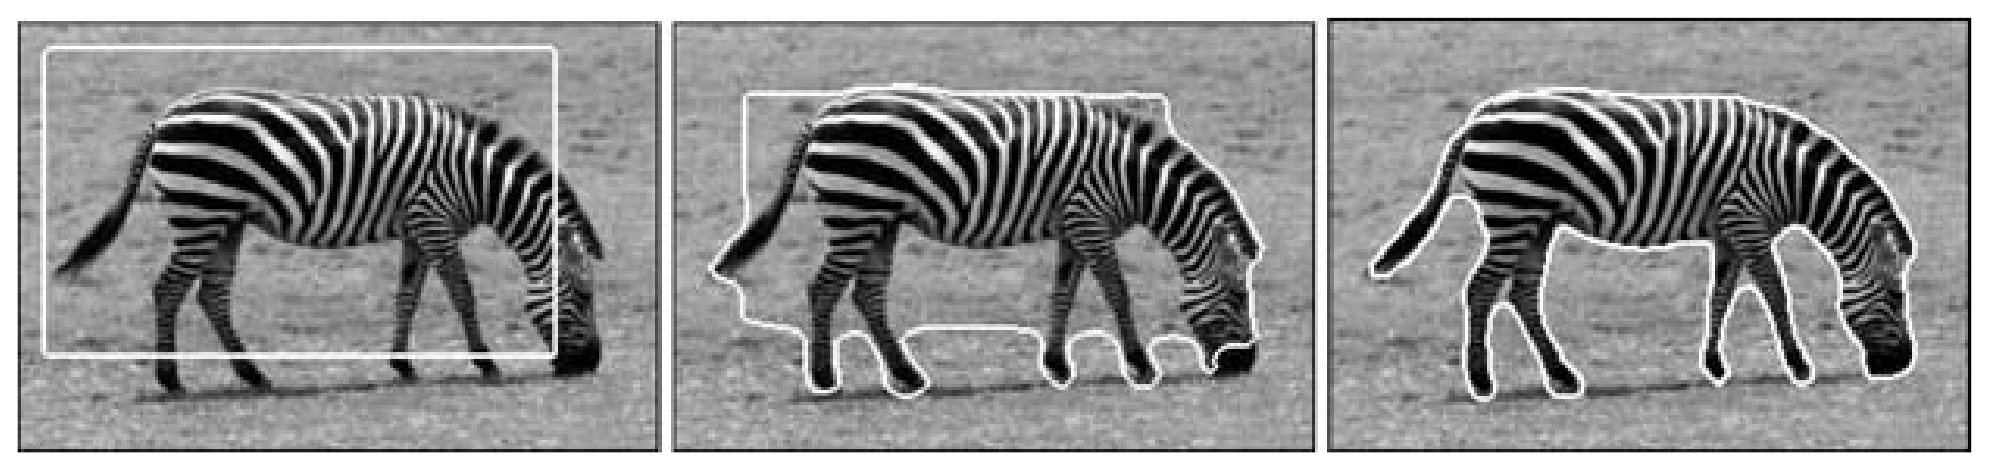
\includegraphics[width=\textwidth]{images/honorable-mentions-5.png}
    \end{center}
    \vspace{-0.5\baselineskip}
    \centering
    \justifying
    \scriptsize Curve evolution for the segmentation of a zebra image using the nonlinear structure tensor and the smoothed intensity (here, a
    rectangle is used as initialization but small circles also lead to a similar result).
    Author: Cremers et al. (2006) \cite{Cremers2006}.
\end{frame}

\begin{frame}{Extensions of the Chan--Vese Model}
    \begin{center}
        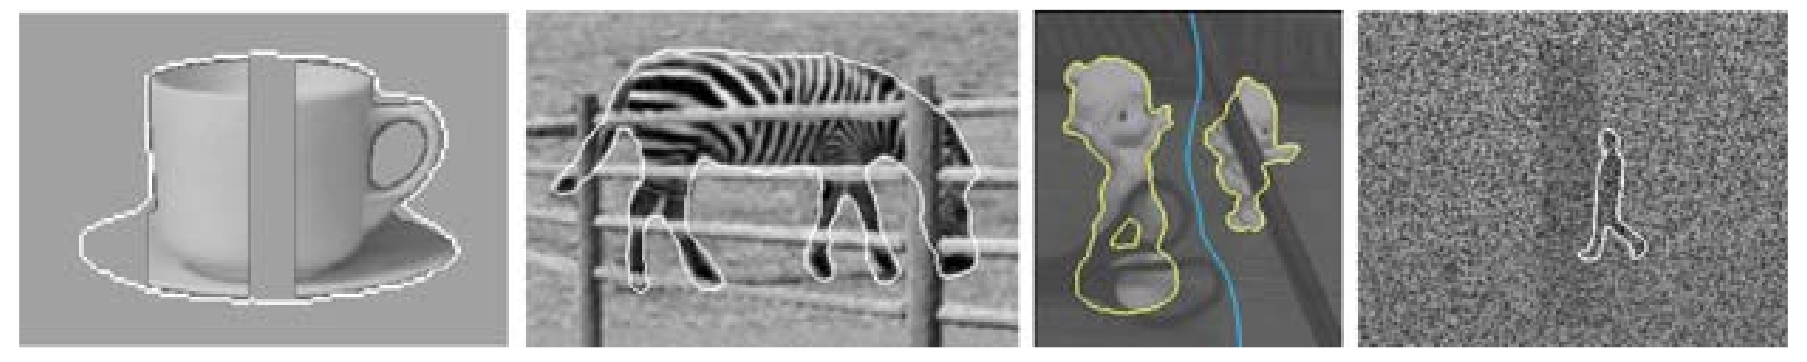
\includegraphics[width=\textwidth]{images/honorable-mentions-6.png}
    \end{center}
    \vspace{-0.5\baselineskip}
    \centering
    \justifying
    \scriptsize Sample segmentations using statistical shape priors. From left to right, the shape priors are a single static shape prior (Rousson and Paragios, 2002), uniformly distributed in the PCA subspace (Rousson, 2004), automatically selected from multiple shape instances (Cremers et al., 2006) and dynamical (Cremers, 2006).
\end{frame}

\section{Concluding Remarks}

\begin{frame}{Concluding Remarks}
    \begin{itemize}
        \item \textbf{Chan and Vese (2001)} introduced an active contour model, that did not rely on gradient computation, based on \emph{Mumford--Shah segmentation} and level set methods. 
        \item Robust to noise; no need for initial image smoothing.
        \item Capable of detecting objects with non-gradient and smooth boundaries.
        \item Efficiently identifies interior contours with a single initial curve.
        \item Initial curve placement is flexible; does not need to encircle the target objects.
    \end{itemize}
\end{frame}

\section{References}

\begin{frame}[allowframebreaks]
    \scriptsize
    \begin{thebibliography}{99}
        \bibitem{ChanVese} T.F. Chan and L.A. Vese,
        \emph{Active contours without edges},
        IEEE Transactions on Image Processing, vol. 10, no. 2, pp. 266-277, 2001, doi: \href{https://doi.org/10.1109/83.902291}{10.1109/83.902291}.

        \bibitem{Caselles} V. Caselles, R. Kimmel, and G. Sapiro,
        \emph{On geodesic active contours},
        International Journal of Computer Vision, vol. 22, pp. 61–79, 1997, doi: \href{https://doi.org/10.1023/A:1007979827043}{10.1023/A:1007979827043}.

        \bibitem{Adalsteinsson} D. Adalsteinsson and J.A. Sethian,
        \emph{A Fast Level Set Method for Propagating Interfaces},
        Journal of Computational Physics, vol. 118, no. 2, pp. 269-277, 1995, doi: \href{https://doi.org/10.1006/jcph.1995.1098}{10.1006/jcph.1995.1098}.

        \bibitem{Kichenassamy} S. Kichenassamy, A. Kumar, P. Olver, A. Tannenbaum, and A. Yezzi,
        \emph{Gradient flows and geometric active contour models},
        Proceedings of IEEE International Conference on Computer Vision, pp. 810-815, 1995, doi: \href{https://doi.org/10.1109/ICCV.1995.466855}{10.1109/ICCV.1995.466855}.

        \bibitem{Adalsteinsson} D. Adalsteinsson and J.A. Sethian,
        \emph{A Fast Level Set Method for Propagating Interfaces},
        Journal of Computational Physics, vol. 118, no. 2, pp. 269-277, 1995, doi: \href{https://doi.org/10.1006/jcph.1995.1098}{10.1006/jcph.1995.1098}.

        \bibitem{Malladi1993}
        R. Malladi, J. A. Sethian, and B. C. Vemuri,
        \emph{A topology independent shape modeling scheme},
        in Proc. SPIE Conf. Geometric Methods Computer Vision II, vol. 2031, San Diego, CA, 1993, pp. 246--258.

        \bibitem{Kass1988}
        M. Kass, A. Witkin, and D. Terzopoulos,
        \emph{Snakes: Active contour models},
        Int. J. Comput. Vis., vol. 1, pp. 321--331, 1988.

        \bibitem{Osher1988} S. Osher and J.A. Sethian,
        \emph{Fronts propagating with curvature-dependent speed: Algorithms based on Hamilton-Jacobi formulations},
        Journal of Computational Physics, vol. 79, no. 1, pp. 12-49, 1988, doi: \href{https://doi.org/10.1016/0021-9991(88)90002-2}{10.1016/0021-9991(88)90002-2}.

        \bibitem{MumfordShah} D. Mumford and J. Shah,
        \emph{Boundary detection by minimizing functionals},
        IEEE CVPR, vol. 17, pp. 22-26, 1985.

        \bibitem{Zhao1996} H.-K. Zhao, T. Chan, B. Merriman, and S. Osher,
        \emph{A variational level set approach to multiphase motion},
        in J. Comput. Phys., vol. 127, 1996, pp. 179--195.

        \bibitem{Chan2000}
        T. F. Chan, B. Sandberg, and L. A. Vese,
        \emph{Active Contours Without Edges for Vector-Valued Images},
        Journal of Visual Communication and Image Representation, vol. 11, pp. 130--141, 2000.
        Available: \url{http://dx.doi.org/10.1006/jvci.1999.0442}

        \bibitem{Rousson2002} M. Rousson and N. Paragios,
        \emph{Shape Priors for Level Set Representations}, in Computer Vision --- ECCV 2002, A. Heyden, G. Sparr, M. Nielsen, and P. Johansen, Eds. Berlin, Heidelberg: Springer Berlin Heidelberg, 2002, pp. 78--92.

        \bibitem{Brox2004} T. Brox and J. Weickert,
        \emph{Level Set Based Image Segmentation with Multiple Regions},
        in Pattern Recognition, C. E. Rasmussen, H. H. B{\"u}lthoff, B. Sch{\"o}lkopf, and M. A. Giese, Eds. Berlin, Heidelberg: Springer Berlin Heidelberg, 2004, pp. 415--423, doi: \href{https://doi.org/10.1007/978-3-540-28649-3_51}{10.1007/978-3-540-28649-3\_51}.

        \bibitem{Cremers2006} D. Cremers,
        \emph{Dynamical statistical shape priors for level set-based tracking}, IEEE Transactions on Pattern Analysis and Machine Intelligence, vol. 28, no. 8, pp. 1262-1273, 2006, doi: \href{https://doi.org/10.1109/TPAMI.2006.161}{10.1109/TPAMI.2006.161}.

        \bibitem{getreuer} P. Getreuer,
        \emph{Chan-Vese Segmentation},
        Image Processing On Line, vol. 2, pp. 214--224, 2012.
        Available: \url{https://doi.org/10.5201/ipol.2012.g-cv}

        \bibitem{yo} Martínez, C. (2021).
        \emph{Aplicación de la visión por computadora en el análisis de microestructuras y la obtención de relaciones estructura - propiedad}. Universidad de los Andes.
        Retrieved from
        \url{http://hdl.handle.net/1992/51616} ([Online; accessed 25.06.2024]).

        \bibitem{Pascal2023} P. Pascal,
        \emph{Differential equations in computer vision, Lecture 25: Self-snakes and Active Contours},
        Universität des Saarlandes, 2023.

        \bibitem{wiki:LipschitzContinuity}
        {Wikipedia contributors},
        \emph{Lipschitz continuity --- {W}ikipedia{,} The Free Encyclopedia},
        Retrieved from
        \url{https://en.wikipedia.org/wiki/Lipschitz_continuity} ([Online; accessed 23.06.2024]).

        \bibitem{wiki:heaviside}
        {Wikipedia contributors},
        \emph{Heaviside step function --- {W}ikipedia{,} The Free Encyclopedia},
        Retrieved from
        \url{https://en.wikipedia.org/wiki/Heaviside_step_function} ([Online; accessed 23.06.2024]).

        \bibitem{wiki:dirac}
        {Wikipedia contributors},
        \emph{Dirac delta function --- {W}ikipedia{,} The Free Encyclopedia},
        Retrieved from
        \url{https://en.wikipedia.org/wiki/Dirac_delta_function} ([Online; accessed 23.06.2024]).

        \bibitem{viso.ai}
        {Viso.ai},
        \emph{Image Segmentation with Deep Learning (Guide)},
        Retrieved from
        \url{https://viso.ai/deep-learning/image-segmentation-using-deep-learning/} ([Online; accessed 25.06.2024]).

        \bibitem{brats} N. Alarcon,
        \emph{Automatically Segmenting Brain Tumors with AI}, NVIDIA Developer Blog,
        Retrieved from
        \url{https://developer.nvidia.com/blog/automatically-segmenting-brain-tumors-with-ai/} ([Online; accessed 25.06.2024]).

        \bibitem{imagej} J. Eglinger,
        \emph{Texture Segmentation}, image.sc Forum,
        Retrieved from
        \url{https://forum.image.sc/t/texture-segmentation/69785} ([Online; accessed 25.06.2024]).
    \end{thebibliography}
\end{frame}

\begin{frame}{Appendix}
    \hypertarget{LargerDiracDelta}{}
    \hyperlink{SmallerDiracDelta}{
        \hfil\makebox[\textwidth][c]{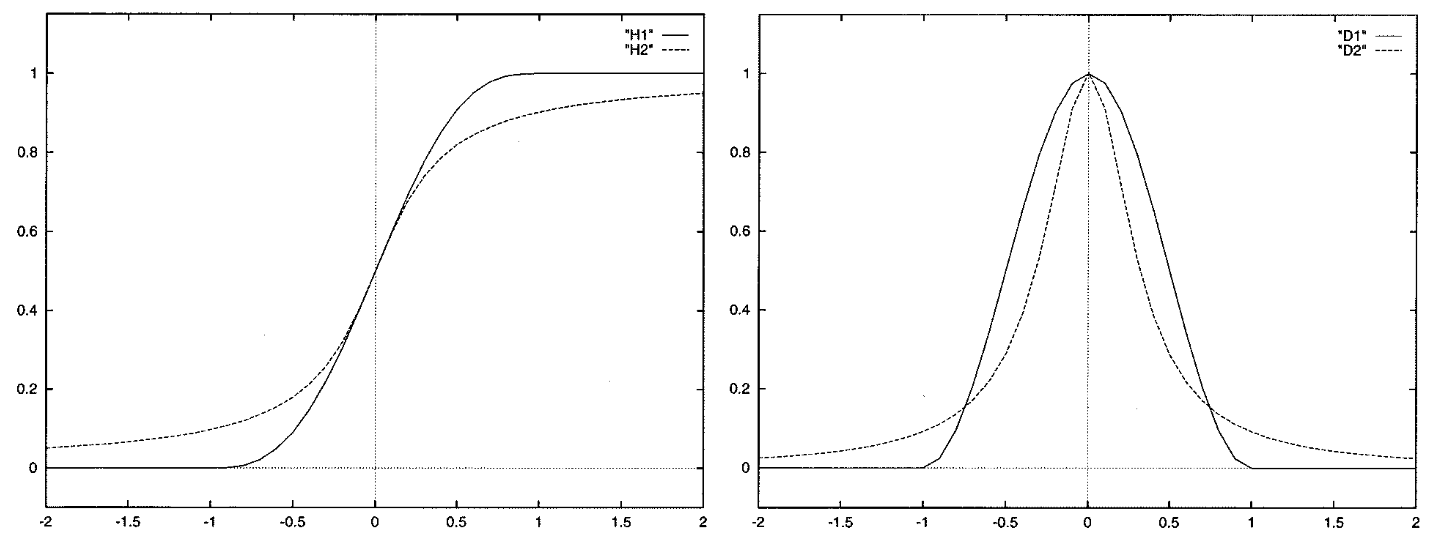
\includegraphics[width=1.2\textwidth]{images/heaviside-regularized.png}}}
    \vfill
    \scriptsize Two different regularizations of the (left) heaviside function $H$ and (right) delta function $\delta_0$ \cite{ChanVese}.
\end{frame}

\end{document}